\documentclass[12,twoside]{TFG-GM}
%\usepackage[active]{srcltx}
\usepackage{amsthm,amsmath,amssymb,amsfonts,amscd}
\usepackage{graphicx}
\usepackage{enumerate}
\usepackage[all]{xy}
\usepackage{booktabs}
%\usepackage[usenames]{xcolor}
%\usepackage{fancyhdr}

%%%%%Author packages if necessary
\usepackage{hyperref}
\usepackage[spanish]{babel}

\usepackage[utf8]{inputenc}
\usepackage[T1]{fontenc}
\usepackage{environ}
\usepackage{float}
\usepackage{tikz}
%\usetikzlibrary{arrows}
\usetikzlibrary{positioning}
\usetikzlibrary{matrix,decorations.pathreplacing,calc}
\usepackage{pgfplots}
\pgfplotsset{compat=1.10}

\usepackage[nottoc]{tocbibind} %Adds "References" to the table of contents

\usepackage{neuralnetwork}
\usepackage{xcolor}
\usepackage{chronology}

%\usepackage[demo]{graphicx}
\usepackage{caption}
\usepackage{subcaption}
\usepackage{wrapfig}
\usepackage[nottoc]{tocbibind}
\usepackage{enumitem}
\setlist{  
  listparindent=\parindent,
  parsep=0pt,
}



% Theorem Environments: add extra ones at the end if you need it.

\newtheorem*{theoremA}{Theorem A}
\newtheorem{theorem}{Theorem}[section]

\newtheorem{proposition}[theorem]{Proposition}
\newtheorem{lemma}[theorem]{Lemma}
\newtheorem{corollary}[theorem]{Corollary}
\newtheorem{conjecture}[theorem]{Conjecture}

\theoremstyle{definition}
\newtheorem{definition}[theorem]{Definición}
\newtheorem{example}[theorem]{Example}

\theoremstyle{remark}
\newtheorem{remark}[theorem]{Remark}
\newtheorem*{remarknonumber}{Remark}
\newtheorem{observation}[theorem]{Observation}




%%%%%%%%%%%%%%%%%%
% macros/abbreviations: Include here your own.
%%%%%%%%%%%%%%%%%%

\newcommand{\N}{\ensuremath{\mathbb{N}}}
\newcommand{\norm}[1]{\left\lVert#1\right\rVert}


\DeclareCaptionType{equ}[][]
\DeclareCaptionLabelFormat{nospace}{#1 #2}
\captionsetup[equ]{name=Ecuación ,labelformat=nospace,labelsep=period}

\setcounter{secnumdepth}{3}
%%%%%%%%%%%%%%%%%%
% tikz config
%%%%%%%%%%%%%%%%%%


\tikzset{basic/.style={draw,fill=blue!20,text width=1em,text badly centered}}
\tikzset{input/.style={basic,circle}}
\tikzset{weights/.style={basic,rectangle}}
\tikzset{functions/.style={basic,circle,fill=blue!10}}
\tikzstyle{arrow}=[draw, -latex]

\makeatletter
\newsavebox{\measure@tikzpicture}
\NewEnviron{scaletikzpicturetowidth}[1]{%
  \def\tikz@width{#1}%
  \def\tikzscale{1}\begin{lrbox}{\measure@tikzpicture}%
  \BODY
  \end{lrbox}%
  \pgfmathparse{#1/\wd\measure@tikzpicture}%
  \edef\tikzscale{\pgfmathresult}%
  \BODY
}
\makeatother



 \pgfkeys{tikz/mymatrixenv/.style={decoration=brace,every left delimiter/.style=    {xshift=3pt},every right delimiter/.style={xshift=-3pt}}}
 \pgfkeys{tikz/mymatrix/.style={matrix of math nodes,left delimiter=[,right delimiter=    {]},inner sep=2pt,column sep=1em,row sep=0.5em,nodes={inner sep=0pt}}}
 \pgfkeys{tikz/mymatrixbrace/.style={decorate,thick}}

\newcommand\mymatrixbraceoffseth{0.5em}
 \newcommand\mymatrixbraceoffsetv{0.2em}
 
\newcommand*\mymatrixbracetop[4][mtr]{
\draw[mymatrixbrace] ($(#1.north west)!(#1-1-#2.north west)!(#1.north east)+(0,\mymatrixbraceoffsetv)$)
    -- node[above=2pt] {#4} 
    ($(#1.north west)!(#1-1-#3.north east)!(#1.north east)+(0,\mymatrixbraceoffsetv)$);
}

\newcommand*\mymatrixbraceleft[4][mtr]{
 \draw[mymatrixbrace] ($(#1.north east)!(#1-#2-1.north east)!(#1.south east)+    (\mymatrixbraceoffseth,0)$)
    -- node[right=2pt] {#4} 
     ($(#1.north east)!(#1-#3-1.south east)!(#1.south east)+    (\mymatrixbraceoffseth,0)$);
}



% Body of document

\titol{ Wordnet y Deep Learning: Una posible unión}
\titolcurt{}
\authorStudent{Raquel Leandra Pérez Arnal}
\supervisors{Dario Garcia Gasulla y Claudio Ulises Cortés García}
\monthYear{Enero, 2017}

%\msc[2010]{Primary  	55M25, 57P10, Secondary 55P15, 57R19, 57N15.}

\paraulesclau{Convolutional Neural Network, Wordnet, Imagenet, Transfer Learning}
\agraiments{
Gracias a Dario y Ulises por ser mis supervisores. Gracias a Ferran y Armand por ayudarme cuando tenía dudas. Gracias a mis amigos por apoyarme cuando estaba desbordada de trabajo y por leerse los distintos borradores que hice cuando estaba redactando el documento.}


\abstracteng{Convolutional neural networks (CNN) are representation learning techniques that achieve
state-of-the-art performance on almost every image-related, machine learning task. Applying the representation languages build by these models to tasks beyond the one they were
originally trained for is a field of interest known as transfer learning for feature extraction. In this work we will study a Full-Network Embedding made ussing transfer learning from a deep convolutional neural network trained for image classification ussing the dataset of Imagenet and it's rellation with different synsets of Wordnet. }

%%%%%%%%%


\begin{document}



\pgfmathdeclarefunction{gauss}{2}{\pgfmathparse{1/(#2*sqrt(2*pi))*exp(-((x-#1)^2)/(2*#2^2))}%
}


\maketitle

\tableofcontents
%\tableofcontents
\newpage

\section{Introducción}

Uno de los campos de estudio en alza del momento es el de \textit{Machine Learning}, una rama de la inteligencia artificial que da a ciertos programas la habilidad de aprender autónoma-mente a partir de datos. Al no programar de forma directa los programas, sino entrenados, dentro de este campo una de las mayores incógnitas es descubrir por que algunos algoritmos toman ciertas decisiones en vez de otras. 

En este trabajo echaremos una ojeada dentro de una red convolucional profunda y estudiaremos las diferentes relaciones que se pueden encontrar entre una red convolucional entrenada con el conjunto de datos de imagenet y los \textit{synsets} de \textit{wordnet}.
Todo esto basándonos en el trabajo presentado en \cite{fne}.  

Para ello empezaremos explicando a nivel general que son una red neuronal, una red convolucional y \textit{transfer learning} en la sección \ref{sec:conocimientosprevios}. Seguidamente explicaremos el contenido del paper \cite{fne} y que son \textit{Wordnet} e \textit{Imagenet} (Sección \ref{sec:trabajorelacionado}).
Una vez explicadas las bases en las que se fundamenta el trabajo, haremos un análisis de un \textit{Full Network Embedding} generado a partir de una red convolucional entrenada con un conjunto de datos de \textit{Imagenet} y estudiaremos las relaciones encontradas entre el \textit{embedding} y unos \textit{synsets} seleccionados (Secciones \ref{sec:enfoque} y \ref{sec:analisis}). Finalmente explicaremos las conclusiones obtenidas a partir de este estudio.    

\section{Conocimientos previos}
\label{sec:conocimientosprevios}
%\subsection{Machine Learning}
%%- Que es ml y por que está de moda. 
%%- Un poco de historia
%En los últimos años(fecha) ha estado en alza todo lo relacionado con \textit{Machine Learning}, pero, que es realmente machine learning? 
%Machine Learning es una aplicación de la Inteligencia Artificial que provee sistemas de la habilidad de mejorar a partir de una experiencia sin ser explícitamente programados para ello. 
%
%Su crecimiento se debe a: 
%\begin{itemize}
%\item Aumento de la capacidad computacional de los ordenadores. 
%\item Aumento de la cantidad de datos disponibles, junto la necesidad de analizarlos. 
%\end{itemize}
%
%En nuestro caso concreto nos centraremos en la aplicación de diversos métodos de ML a el problema de clasificación de imágenes. 


\subsection{Redes neuronales}
Una \textbf{red neuronal} es un modelo computacional de aprendizaje inspirado en la forma de procesar información de las neuronas del cerebro. Las redes neuronales han generado una significativa cantidad de investigación e industria gracias a sus resultados en reconocimiento del habla, visión por computador y procesamiento de texto. Para dejar claro su funcionamiento explicaremos primero el funcionamiento de una sola neurona, para después unirlo con la organización por capas de varias neuronas y finalmente explicar el algoritmo de \textit{backpropagation}, mediante el cual se entrenan estos modelos de aprendizaje automático. 

\subsubsection{Una neurona}

\begin{definition} 
La unidad de computación básica de una red neuronal es una \textbf{neurona}, también llamada nodo o unidad. Ésta, recibe una conjunto de entradas sobre la que se aplica una función para generar una salida.
\end{definition}
Cada entrada (\textbf{x}) tiene asociado un peso (\textbf{w}), que es aprendido en base a su importancia relativa a otras entradas, a la salida y al objetivo de la red. La neurona  aplica una función (\textbf{f}) a la suma ponderada de las entradas. 
%\begin{center}
%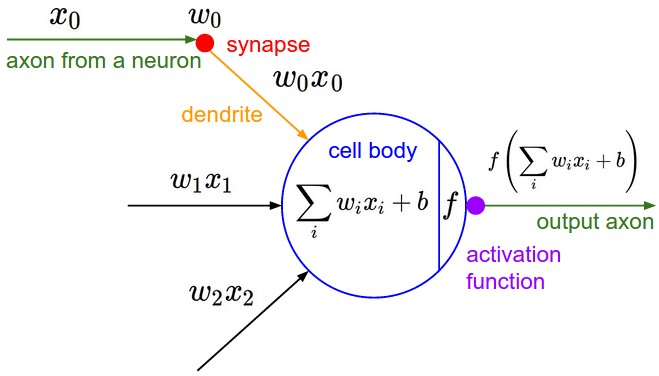
\includegraphics[width=0.5\textwidth]{Images/neuron_model.jpeg} 
%\end{center}

Además de los elementos ya comentados tendremos un término de sesgo ($w_0$), cuyo objetivo es proveer cada neurona con un valor entrenable que no dependa de la entrada y facilitar el ajuste del modelo a los datos. 

La salida de la neurona (\textbf{y}) se calculara de la siguiente manera: 

$$
\mathbf{y}(\mathbf{x},\mathbf{w}) = f \left(\sum_{i=1}^N \omega_i x_i + w_0 \right) 
$$

Llamaremos a \textbf{f} la \textbf{función de activación}, es una función (no lineal), generalmente diferenciable, cuyo propósito es introducir no linealidad a la salida de la neurona. Ésto permite adaptar el modelo a problemas reales, puesto a que estos generalmente requieren relaciones no lineales. 

En la figura \ref{fig:perceptron} podemos ver un ejemplo visual del comportamiento de una sola neurona.
\begin{figure}[H]
\centering
 \begin{tikzpicture}
        \node[functions] (center) {$f$};
        \node[below of=center,font=\scriptsize,text width=4em] {Función de activación};

        \node[right of=center] (right) {};
            \path[draw,arrow] (center) -- (right);
        \node[functions,left=3em of center,text width=3em ] (left) {$\sum w_i x_i$};
            \path[draw,arrow] (left) -- (center);
        \node[weights,left=3em of left] (2) {$w_2$} -- (2) node[input,left of=2] (l2) {$x_2$};
            \path[draw,arrow] (l2) -- (2);
            \path[draw,arrow] (2) -- (left);
        \node[below of=2] (dots) {$\vdots$} -- (dots) node[left of=dots] (ldots) {$\vdots$};
        \node[weights,below of=dots] (n) {$w_n$} -- (n) node[input,left of=n] (ln) {$x_n$};
            \path[draw,arrow] (ln) -- (n);
            \path[draw,arrow] (n) -- (left);
        \node[weights,above of=2] (1) {$w_1$} -- (1) node[input,left of=1] (l1) {$x_1$};
            \path[draw,arrow] (l1) -- (1);
            \path[draw,arrow] (1) -- (left);
        \node[weights,above of=1] (0) {$w_0$} -- (0) node[input,left of=0] (l0) {$1$};
            \path[draw,arrow] (l0) -- (0);
            \path[draw,arrow] (0) -- (left);
        \node[below of=ln,font=\scriptsize] {Pesos};
        \node[below of=n,font=\scriptsize] { Entrada};
    \end{tikzpicture}
    \caption{Ejemplo de una neurona \label{fig:perceptron}}
\end{figure}



Las funciones de activación más utilizadas son: 

\begin{itemize}
\item Sigmoide: $f(x)=\frac{1}{1+e^{-x}}$
\begin{figure}[H]
\centering
%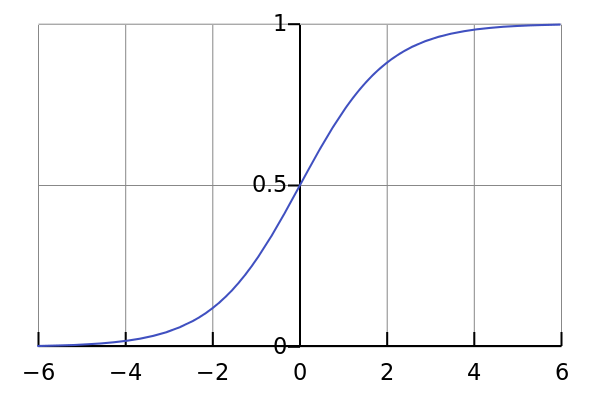
\includegraphics[width=0.5\textwidth]{Images/sigmoid.png} 
\begin{scaletikzpicturetowidth}{0.5\textwidth}
\begin{tikzpicture}[scale=\tikzscale]
    \begin{axis}[
        legend pos=north west,
        axis x line=middle,
        axis y line=middle,
        y tick label style={/pgf/number format/fixed,
                            /pgf/number format/fixed zerofill,
                            /pgf/number format/precision=1},
        grid = major,
        width=16cm,
        height=8cm,
        grid style={dashed, gray!30},
        xmin=-4,     % start the diagram at this x-coordinate
        xmax= 4,     % end   the diagram at this x-coordinate
        ymin= 0,     % start the diagram at this y-coordinate
        ymax= 1,     % end   the diagram at this y-coordinate
        %axis background/.style={fill=white},
        xlabel=$t$,
        ylabel=sig$(t)$,
        tick align=outside,
        enlargelimits=true]
      % plot the stirling-formulae
      \addplot[domain=-5:5, black, ultra thick,samples=500] {1/(1+exp(-1*x))};
      \addlegendentry{sig$(t)=\frac{1}{1+e^{-t}}$}
    \end{axis}
\end{tikzpicture}
\end{scaletikzpicturetowidth}
%\caption{Ejemplo de red neuronal}
\end{figure}
\item Tanh: $f(x)=\frac{2}{1+e^{-2x}}-1$
\begin{figure}[H]
\centering
%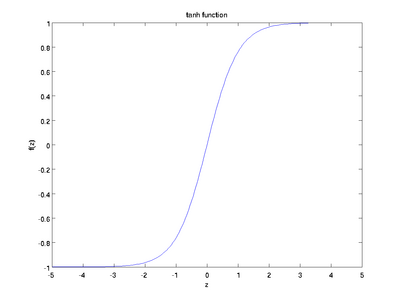
\includegraphics[width=0.5\textwidth]{Images/tanh.png} 
\begin{scaletikzpicturetowidth}{0.5\textwidth}
\begin{tikzpicture}[scale=\tikzscale]
    \begin{axis}[
        legend pos=north west,
        axis x line=middle,
        axis y line=middle,
        y tick label style={/pgf/number format/fixed,
                            /pgf/number format/fixed zerofill,
                            /pgf/number format/precision=1},
        grid = major,
        width=16cm,
        height=8cm,
        grid style={dashed, gray!30},
        xmin=-4,     % start the diagram at this x-coordinate
        xmax= 4,     % end   the diagram at this x-coordinate
        ymin= -1,     % start the diagram at this y-coordinate
        ymax= 1,     % end   the diagram at this y-coordinate
        %axis background/.style={fill=white},
        xlabel=$x$,
        ylabel=$tanh(x)$,
        tick align=outside,
        enlargelimits=true]
      % plot the stirling-formulae
      \addplot[domain=-5:5, black, ultra thick,samples=500] {2/(1+exp(-2*x)) - 1};
      \addlegendentry{$tanh(x)=\frac{2}{1+e^{-2x}}-1$}
    \end{axis}
\end{tikzpicture}
\end{scaletikzpicturetowidth}
\end{figure}

%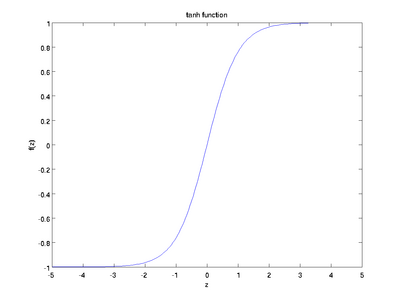
\includegraphics[scale=1]{Images/tanh.png} 
\item ReLU: $f(x)=max(0,x)$. Puesto que no es diferenciable en el cero, para poder utilizar \textit{back-propagation} se suele tomar $f'(0)=x_0$ siendo $x_0$ un valor arbitrario. 

\begin{figure}[H]
\centering
%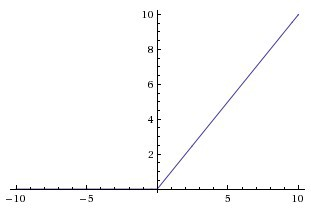
\includegraphics[width=0.5\textwidth]{Images/relu.jpeg} 
\begin{scaletikzpicturetowidth}{0.5\textwidth}
\begin{tikzpicture}[scale=\tikzscale]
    \begin{axis}[
        legend pos=north west,
        axis x line=middle,
        axis y line=middle,
        y tick label style={/pgf/number format/fixed,
                            /pgf/number format/fixed zerofill,
                            /pgf/number format/precision=1},
        grid = major,
        width=16cm,
        height=8cm,
        grid style={dashed, gray!30},
        xmin=-4,     % start the diagram at this x-coordinate
        xmax= 4,     % end   the diagram at this x-coordinate
        ymin= 0,     % start the diagram at this y-coordinate
        ymax= 4,     % end   the diagram at this y-coordinate
        %axis background/.style={fill=white},
        xlabel=$x$,
        ylabel=$relu(x)$,
        tick align=outside,
        enlargelimits=true]
      % plot the stirling-formulae
      \addplot[domain=-5:5, black, ultra thick,samples=500] {max(0,x)};
      \addlegendentry{$f(x)=max(0,x)$}
    \end{axis}
\end{tikzpicture}
\end{scaletikzpicturetowidth}
\end{figure}
%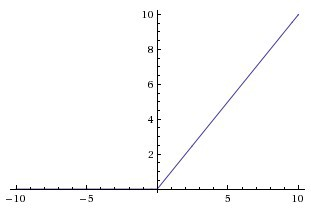
\includegraphics[scale=1]{Images/relu.png} 
\end{itemize}


Dotando una neurona de una función de pérdida en la salida podríamos convertirla en un clasificador lineal, pero la verdadera potencia del método viene dada al unir diversas neuronas en lo que llamaremos capas.


\subsubsection{Organización por capas}
Las redes neuronales se modelizan como una colección de neuronas conectadas en un grafo acíclico, comúnmente organizado por capas. El tipo más común de capa es la capa completa (\textit{fully-connected layer}), en el que todas las neuronas de una capa están conectadas con todas las neuronas de la capa posterior a ésta, mientras que no comparten ninguna conexión con las de su propia capa, como muestra la figura \ref{fig:red neuronal}. %Si tenemos diversas capas ocultas diremos que se trata de una red profunda (\textit{deep network}).
\begin{figure}[H]
\begin{center}
\begin{neuralnetwork}[height=5]
		\newcommand{\nodetextclear}[2]{}
		\newcommand{\nodetextx}[2]{$x_#2$}
		\newcommand{\nodetexty}[2]{$y_#2$}
		\newcommand{\nodetextw}[2]{$w_#2^#1$}
		\inputlayer[count=3, bias=true, title=Capa \\de entrada, text=\nodetextx]
		\hiddenlayer[count=4, bias=true, title=Capa \\ oculta 1, text=\nodetextw] \linklayers
		\hiddenlayer[count=4, bias=true, title=Capa \\ oculta 2, text=\nodetextw] \linklayers
		\outputlayer[count=3, title=Capa\\ de salida, text=\nodetexty] \linklayers
	
	\end{neuralnetwork}
	
\end{center}
\caption{Ejemplo de red neuronal compuesta por capas completas\label{fig:red neuronal}}
\end{figure}
La red neuronal más básica la podemos dividir en: 
\begin{enumerate}
\item Neuronas de entrada: Proveen la red de información del exterior, consisten en los datos de entrada, todo su conjunto se conoce como la capa de entrada. 
\item Neuronas ocultas: Las neuronas ocultas no tienen conexión directa con el exterior. Solo calculan y transfieren información de la entrada a la salida. La colección de las neuronas ocultas se denomina las capas ocultas.
\item Neuronas de salida: Colectivamente denominados capa de salida y son responsables de generar la salia de la red neuronal calculada a partir de la entrada y procesada por varias capas. 
\end{enumerate}

Matemáticamente la notación (tomada de \cite{Bishop2006}) varía ligeramente al añadir capas. Si tenemos una muestra de tamaño $N$ y una red con $M$ capas,definimos las activaciones ($a_j^{(k)}$) para cada neurona $j$ de la capa $k$ como: 
\begin{equ}[H]
\begin{equation*}
a_j^{(k)}(\mathbf{x},\mathbf{w}) = \sum_{i=1}^N w_{ji}^{(k)}x_i + w_{j0}^{(k)}
\end{equation*}
\caption{\label{eq:activaciones}}
\end{equ}
Donde $w_ji$ es el peso que va de la neurona $i$ a la neurona $j$ y $w_j0$ es el sesgo.

 Si tomamos $z_j^{(k)} = f(a_j^{(k)})$ podemos expresar las activaciones de la siguiente capa como: 
 \begin{equ}[H]
\begin{equation*}
a_j^{(k+1)}(\mathbf{x},\mathbf{w}) = \sum_{i=1}^N w_{ji}^{k}z_j^{(k)} + w_{j0}^{(k)}
\end{equation*}
\caption{\label{eq:activacionesv1}}
\end{equ}

Después de procesar todas las capas la salida de la red sería:

 \begin{equ}[H]
\begin{equation*}
\mathbf{y}(\mathbf{x},\mathbf{w}) = \mathbf{a}^{(M)} = \sum_{i=1}^N w_{ji}^{(M-1)}z_j^{(M -1)} + w_{j0}^{(M-1)} = \sum_{i=1}^N w_{ji}^{(M-1)}\left(\sum_{i=1}^N w_{ji}^{(M-2)}z_j^{(M-2)} + w_{j0}^{(M-2)} \right) + w_{j0}^{(M-1)}
\end{equation*}
\caption{\label{eq:activacionesv2}}
\end{equ}
Donde, para calcular la salida, habría que calcular todos los sumatorios encadenados hasta llegar a la entrada.  

De esta forma nos queda una estructura formada por pesos ordenados en distintos tipos de capas. Cada peso de la red es un parámetro que necesitamos que la red aprenda, y de esta forma corresponda con el resultado esperado (con mayor o menor error). Para ello se utiliza el algoritmo de \textit{backpropagation}, que explicaremos en el siguiente apartado.

\subsubsection{Entrenar la red: Backpropagation}\label{sec:backpropagation}
Finalmente, queda explicar como entrenar los distintos parámetros (i.e. pesos) para que se adapten a los datos, para ello se utiliza \textbf{backpropagation}.

La idea general del algoritmo consiste en obtener las derivadas parciales de la función de error respecto a los pesos. Como el error sólo se puede computar a la salida, para poder obtener las de los parámetros intermedios utiliza la regla de la cadena. El objetivo del algoritmo es, una vez tengamos las derivadas, utilizar un algoritmo de minimización sobre la función de error para obtener los valores entrenados de los pesos.

Sea $E(\mathbf{w})$ nuestra función de error,que depende de los pesos $\mathbf{w}$, y $\mathbf{t}$ el vector objetivo, es decir, los valores que debería dar la red neuronal dada la entrada $\mathbf{X} = \{\mathbf{x}_1, ..., \mathbf{x}_N\}$. 

Si tomamos el error de mínimos cuadrados tenemos:  
\begin{equ}[H]
\begin{equation*}
E(\mathbf{w}) = \frac{1}{2}\sum_{n=1}^N \norm{\mathbf{y}(\mathbf{x}_n,\mathbf{w}) - \mathbf{t}_n}^2
\end{equation*}
\caption{\label{eq:error}}
\end{equ}

Que, como vimos en la ecuación \ref{eq:activacionesv2}, depende de los pesos de todas las capas. Esta estructura nos dificulta minimizar la función de una forma eficiente.

Para facilitar la notación, definimos $z_0 = 1$, $y_{nk} = y_k(\mathbf{x}_n, \mathbf{w})$ y $E_n(w) = \frac{1}{2} \norm{\mathbf{y}(\mathbf{x}_n,\mathbf{w}) - \mathbf{t}_n}^2$, de esta forma tenemos:
 
\begin{equ}[H]
\begin{align*}
a_j^{(k)} &= \sum_{i=0}^N w_{ji}z_i^{(k)} 
\end{align*}
\caption{Activación de la neurona  $j$ de la capa $k$\label{eq:simplificacionactivacion}}
\end{equ}

\begin{equ}[H]
\begin{align*}
 E_n &= \frac{1}{2} \sum_h (y_{nh} - t_{nh})^2
\end{align*}
\caption{Error en función de la muestra\label{eq:simplificacionerrormuestra}}
\end{equ}

\begin{equ}[H]
\begin{align*}
 E(\mathbf{w}) &= \sum_{n=1}^N E_n(\mathbf{w})
\end{align*}
\caption{Error total\label{eq:simplificacionerrortotal}}
\end{equ}


Donde $a_j^{(k)}$ es la activación de la neurona $j$ de la capa $k$ y el índice $h$ corresponde a cada una de las coordenadas de los vectores $\mathbf{y}$ y $\mathbf{t}$.
 
Para calcular las derivadas de $E(\mathbf{w})$, calcularemos cada una de las de $E_n$ que definimos en la ecuación \ref{eq:simplificacionerrormuestra}. 

Como vemos en la siguiente ecuación:

\begin{equ}[H]
\begin{align*}
\frac{\partial E_n}{\partial w_{ji}^{(k)}} = (y_{nj} - t_{nj})\frac{\partial y_{nj}}{\partial w_{ji}^{(k)}}
\end{align*}
\caption{\label{eq:derivada1}}
\end{equ}
Donde $n$ es el índice de la muestra, $j$ es el índice de la neurona y $k$ es el índice de la capa.

Utilizando la ecuación \ref{eq:activacionesv2}, podemos calcular el valor que corresponde a la derivada del error respecto a los pesos de la última capa (que depende de la penúltima), sin embargo el cálculo de la derivada respecto a los pesos de capas anteriores se dificulta. 

\begin{equ}[H]
\begin{align*}
\frac{\partial E_n}{\partial w_{ji}^{(M)}} = (y_{nj} - t_{nj})z_{j}^{(M-1)}
\end{align*}
\caption{\label{eq:derivada2}}
\end{equ}

Para continuar desarrollando introducimos la siguiente notación: 
\begin{equ}[H]
\begin{align*}
\delta_j^{(k)} = \frac{\partial E_n}{\partial a_j^{(k)}} 
\end{align*}
\caption{\label{eq:delta}}
\end{equ}
Donde las $\delta$ se suelen llamar errores. Además si calculamos la derivada de las activaciones respecto a los pesos utilizando la simplificación de la fórmula \ref{eq:simplificacionactivacion} tenemos:

\begin{equ}[H]
\begin{align*}
\frac{\partial a_j^{(k)}}{\partial w_{ji}^{(k)}} = z_i^{(k)}
\end{align*}
\caption{\label{eq:derivadaactivacion}}
\end{equ}

Utilizando la regla de la cadena sobre $\frac{\partial E_n}{\partial w_{ji}^{(k)}}$ y utilizando \ref{eq:delta} y \ref{eq:derivadaactivacion} tenemos: 

\begin{equ}[H]
\begin{align*}
\frac{\partial E_n}{\partial w_{ji}^{(k)}} = \frac{\partial E_n}{\partial a_j^{(k)}} \frac{\partial a_j^{(k)}}{\partial w_{ji}^{(k)}} = \delta_j^{(k)} z_i^{(k)} 
\end{align*}
\caption{\label{eq:cadena}}
\end{equ}

Utilizando \ref{eq:delta} con los nodos de salida y \ref{eq:error}, tenemos:

\begin{equ}[H]
\begin{align*}
\delta_h^{(M)} = y_h - t_h 
\end{align*}
\caption{\label{eq:finaldelta}}
\end{equ}

El resto de $\delta$s se pueden calcular utilizando la regla de la cadena sobre \ref{eq:delta} y el valor de delta de la capa final \ref{eq:finaldelta}. De esta forma tenemos: 

\begin{equ}[H]
\begin{align*}
\delta_j= \frac{\partial E_n}{\partial a_j} = \sum_{l}  \frac{\partial E_n}{\partial a_l} \frac{\partial a_l}{\partial a_j}
\end{align*}
\caption{\label{eq:finaldeltacadena}}
\end{equ}
Donde la $l$ incluye todas las neuronas a las que está conectada $j$.
Finalmente, uniendo todo obtenemos la \textbf{fórmula de backpropagation}:

\begin{equ}[H]
\begin{align*}
\delta_j= f'(a_j) \sum_{l}  w_{lj}\delta_l
\end{align*}
\caption{\label{eq:backprop}}
\end{equ}
En resumen,dada una inicialización aleatoria o con una distribución dada de la red, el algoritmo de \textit{backpropagation} empieza con un \textit{fordward pass} (una evaluación en la que se procesa la entrada desde el principio hasta generar la salida de acuerdo con el estado actual de la red) por toda la red, con el que se calcula la $y_{n}$ y todas las activaciones $a_{ij}^{(k)}$, la predicción dada por la red se compara con la salida esperada ($t_n$) 
y se calcula un error ($\delta$) para los pesos de la salida, luego se propaga este error utilizando \ref{eq:backprop}. Finalmente utilizando \ref{eq:cadena} obtenemos los valores de las derivadas para todos los pesos.

%\textbf{TODO: Añadir un ejemplo, Revisar los índices de las fórmulas (añadir la capa?)}


Una vez calculadas las derivadas, se utiliza el \textit{ Stochastic Gradient Descent}, o otros métodos de minimización, para obtener los valores de los pesos que minimizan el error.
El \textit{ Stochastic Gradient Descent} \cite{Bishop2006} es un método iterativo que, dada una función a minimizar $E(w)$ obtiene un mínimo local. 

Cada nuevo valor para $w^{(i+1)}$ (nótese que en este caso utilizamos el super-índice para indicar la iteración a la que corresponde $w$, no como índice de la capa) se calcula de la siguiente forma (partiendo de una inicialización aleatoria): 
\begin{equ}[H]
\begin{align*}
w^{(i+1)} := w^{(i)} - \lambda \nabla E (w^{(i)})
\end{align*}
\end{equ}
Donde $\lambda$ es un hiper-parámetro a añadir a nuestro modelo y $\nabla E (w^{(i)})$ es el gradiente de $E$, cuyos términos hemos calculado utilizando \textit{backpropagation}.
Nótese que al ser una optimización en un espacio multi-dimensional (por cada capa un peso por neurona, siendo cada peso un parámetro a optimizar), se requiere muchas muestras y ver varias veces cada muestra para minimizar el error. 
\newpage

\subsection{Redes convolucionales}
%- Explicar el problema inicial (clasificación de imágenes) y por que es difícil.
%- Explicar que es una red convolucional 
\begin{definition}
Una \textbf{red convolucional} es una secuencia de capas de diferentes tipos, donde  al menos una de las capas es una capa convolucional. 
\end{definition}
Las redes convolucionales son muy similares a las redes neuronales explicadas en la sección anterior, las mayores diferencias son que contienen un tipo especial de neuronas (las neuronas convolucionales) y que asume explícitamente que la entrada son datos con una estructura concreta (como por ejemplo imágenes), lo que permite añadir ciertas propiedades a la arquitectura. Esto permite hacer un \textit{fordward pass} más eficiente de implementar y reducir significativamente la cantidad de parámetros.

Una neurona convolucional es aquella que opera con una convolución\cite{deeplearningbook}.

\begin{definition} \label{def:convolution}
Una \textbf{convolución} es una aplicación matemática cuya entrada son dos funciones de valores reales (\textbf{x} y \textbf{w}) y cuya salida es otra función (\textbf{s}). 

Usualmente se denota como $s(t) = (x * w)(t) $.

En el contexto de redes convolucionales llamaremos a \textit{x} \textit{entrada}, a \textit{w} kernel y a la salida \textit{s} \textit{feature map}.
\end{definition}

Nótese que la definición no depende de la dimensión del espacio, es decir, que podemos definir una convolución para tantas dimensiones como necesitemos.
En el caso concreto de una imagen \textit{I} (de dos dimensiones) y un kernel \textit{K}, la convolución quedaría como: 
\begin{equ}[H]
\begin{equation*}
S(i,j) = (I * K)(i,j) = \sum_m \sum_n I(i +m, j+n) K(m,n)
\end{equation*}
\caption{Convolución}
\end{equ}


%\begin{center}
%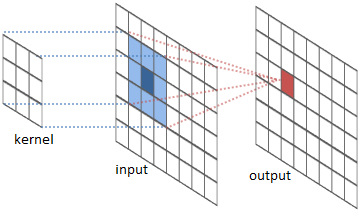
\includegraphics[width = 0.5\textwidth]{Images/convolution2.png} 
%\end{center}
\begin{definition}
Una \textbf{función de kernel} es aquella que cumple: 

\begin{equation*}
K(x,x') = \Phi(x)^T \Phi(x')
\end{equation*}

Donde $x,x' \in X$, siendo $X$ un conjunto, y $\Phi$ es una función de base tal que $\Phi(x)^T \Phi(x') \in \mathbb{R}$. En el caso de las redes convolucionales se suele utilizar un \textit{kernel} lineal. 

\end{definition}
 

Típicamente las neuronas convolucionales tienen una entrada limitada, es decir están conectadas solo a un subconjunto de las neuronas de la capa anterior, de esta forma cada neurona se centra solo en parte de la entrada, lo que significa el aprendizaje de las neuronas individuales cuando hay entradas de muchas dimensiones. En contraste, las neuronas de una capa \textit{fully-connected} están conectadas a todas las neuronas de la capa anterior. %En este caso detallaremos el caso de datos en dos dimensiones, por ser el caso más común y por ser más fácil de entender. Una vez comprendida una convolución 2-dimensional, el lector puede extrapolar a tantas dimensiones como sea necesario.
De esta forma las redes convolucionales reducen la cantidad de parámetros de la red.
%Para definir su conectividad de entrada, las neuronas convolucionales asumen la existencia de una cierta estructura en los datos. 
%Para capturar patrones consistentes, las neuronas convolucionales están conectadas a un conjunto de neuronas de la capa anterior que definen parcelas cuadradas (en el caso de convoluciones de dos dimensiones).



Por su conectividad limitada, las capas convolucionales pueden centrarse en una parcela particular de la entrada. El conjunto de pesos (que sería equivalente al kernel comentado en la definición \ref{def:convolution}) aprendido por esta parcela puede ser relevante para las otras parcelas de la entrada, por tanto, podemos definir neuronas similares que utilicen el mismo kernel, pero que se enfoquen en otra parte de la entrada. Esta idea se conoce como "weight sharing", por que varias neuronas de la misma capa están definidas por un conjunto común de pesos, esto permite tener una considerable cantidad de neuronas utilizando los mismos parámetros. Esto puede ayudar a detectar los mismos patrones en diferentes partes de la entrada. Por ejemplo si tenemos una neurona que detecta ojos, al pasarla por una foto con una cara se activará dos veces.  


\begin{figure}[H]

\begin{center}
%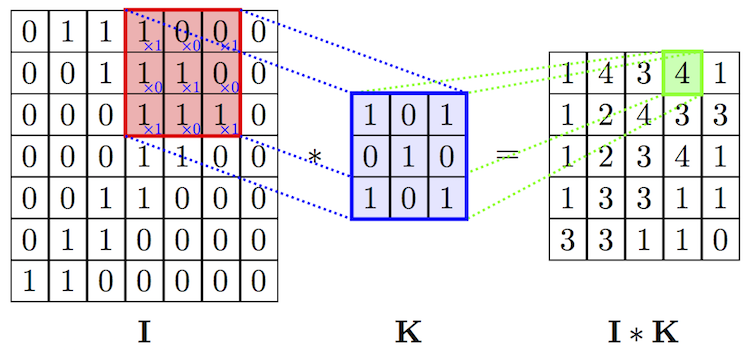
\includegraphics[width = 0.5\textwidth]{Images/convolve.png} 
\begin{tikzpicture}

	\matrix (mtr) [matrix of nodes,row sep=-\pgflinewidth, nodes={draw}]
	{
		0 & 1 & 1 & |[fill=red!30]| 1 & |[fill=red!30]| 0 & |[fill=red!30]| 0 & 0\\
		0 & 0 & 1 & |[fill=red!30]| 1 & |[fill=red!30]| 1 & |[fill=red!30]| 0 & 0\\
		0 & 0 & 0 & |[fill=red!30]| 1 & |[fill=red!30]| 1 & |[fill=red!30]| 1 & 0\\
		0 & 0 & 0 & 1 & 1 & 0 & 0\\
		0 & 0 & 1 & 1 & 0 & 0 & 0\\
		0 & 1 & 1 & 0 & 0 & 0 & 0\\
		1 & 1 & 0 & 0 & 0 & 0 & 0\\
	};

	\draw[very thick, red] (mtr-1-4.north west) rectangle (mtr-3-6.south east);

	\node [below= of mtr-5-4.south] (lm) {$\bf I$};

	\node[right = 0.2em of mtr] (str) {$*$};

	\matrix (K) [right=0.2em of str,matrix of nodes,row sep=-\pgflinewidth, nodes={draw, fill=blue!30}]
	{
		1 & 0 & 1 \\
		0 & 1 & 0 \\
		1 & 0 & 1 \\
	};
	\node [below = of K-3-2.south] (lk) {$\bf K$};

	\node [right = 0.2em of K] (eq) {$=$};

	\matrix (ret) [right=0.2em of eq,matrix of nodes,row sep=-\pgflinewidth, nodes={draw}]
	{
		1 & 4 & 3 & |[fill=green!30]| 4 & 1\\
		1 & 2 & 4 & 3 & 3\\
		1 & 2 & 3 & 4 & 1\\
		1 & 3 & 3 & 1 & 1\\
		3 & 3 & 1 & 1 & 0\\
	};
	\node [below = of ret-4-3.south] (lim) {${\bf I} * {\bf K}$};

	\draw[very thick, green] (ret-1-4.north west) rectangle (ret-1-4.south east);

	\draw[densely dotted, blue, thick] (mtr-1-4.north west) -- (K-1-1.north west);
	\draw[densely dotted, blue, thick] (mtr-3-4.south west) -- (K-3-1.south west);
	\draw[densely dotted, blue, thick] (mtr-1-6.north east) -- (K-1-3.north east);
	\draw[densely dotted, blue, thick] (mtr-3-6.south east) -- (K-3-3.south east);

	\draw[densely dotted, green, thick] (ret-1-4.north west) -- (K-1-1.north west);
	\draw[densely dotted, green, thick] (ret-1-4.south west) -- (K-3-1.south west);
	\draw[densely dotted, green, thick] (ret-1-4.north east) -- (K-1-3.north east);
	\draw[densely dotted, green, thick] (ret-1-4.south east) -- (K-3-3.south east);

	\matrix (K) [right=0.2em of str,matrix of nodes,row sep=-\pgflinewidth, nodes={draw, fill=blue!10}]
	{
		1 & 0 & 1 \\
		0 & 1 & 0 \\
		1 & 0 & 1 \\
	};

	\draw[very thick, blue] (K-1-1.north west) rectangle (K-3-3.south east);

	\node[anchor=south east, inner sep=0.01em, blue] at (mtr-1-4.south east) (xx) {\scalebox{.5}{$\times 1$}};
	\node[anchor=south east, inner sep=0.01em, blue] at (mtr-1-5.south east) (xx) {\scalebox{.5}{$\times 0$}};
	\node[anchor=south east, inner sep=0.01em, blue] at (mtr-1-6.south east) (xx) {\scalebox{.5}{$\times 1$}};
	\node[anchor=south east, inner sep=0.01em, blue] at (mtr-2-4.south east) (xx) {\scalebox{.5}{$\times 0$}};
	\node[anchor=south east, inner sep=0.01em, blue] at (mtr-2-5.south east) (xx) {\scalebox{.5}{$\times 1$}};
	\node[anchor=south east, inner sep=0.01em, blue] at (mtr-2-6.south east) (xx) {\scalebox{.5}{$\times 0$}};
	\node[anchor=south east, inner sep=0.01em, blue] at (mtr-3-4.south east) (xx) {\scalebox{.5}{$\times 1$}};
	\node[anchor=south east, inner sep=0.01em, blue] at (mtr-3-5.south east) (xx) {\scalebox{.5}{$\times 0$}};
	\node[anchor=south east, inner sep=0.01em, blue] at (mtr-3-6.south east) (xx) {\scalebox{.5}{$\times 1$}};

\end{tikzpicture}

\end{center}
\caption{Ejemplo de la forma de operar una convolución sobre una imagen.
\label{fig:conv}
}
\end{figure}

En la figura \ref{fig:conv} podemos ver un ejemplo del funcionamiento de una convolución con un kernel de tamaño 9 sobre una imagen, podemos observar como se comparten los pesos a la hora de calcular el resultado.
Dada una sección de la red, el \textit{kernel} multiplica cada uno de sus valores por el valor correspondiente de ésta, para finalmente, sumar el resultado de todos los productos.


Finalmente queda comentar los tipos de capa más comunes en una red convolucional: 
\begin{itemize}
\item Capa convolucional, capas formadas por neuronas convolucionales, la mayoría de capas de una red convolucional serán de este tipo.
\item Capa \textit{fully-connected}, es una capa donde todas las neuronas están conectadas entre ellas. Se suele utilizar como capa de clasificación. 
\item \textit{Pooling Layer}, consiste en una capa que aplica una reducción matemática a su input (como una media o un max). El objetivo es aportar un cierto grado de invariancia espacial (imágenes equivalentes en diferentes posiciones), además reducen el tamaño de la salida de la capa, lo que provoca una reducción de la complejidad de la red. Un ejemplo de \textit{pooling layer} sería la figura \ref{fig:pooling}.
\end{itemize}

\begin{figure}[h]
\centering
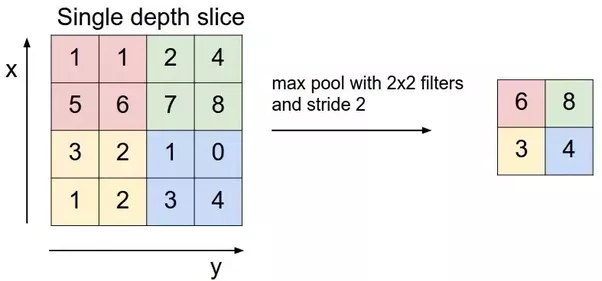
\includegraphics[width = 0.5\textwidth]{Images/pooling1.png} 
\caption{ \label{fig:pooling}}
\end{figure}

Otro concepto que utilizaremos a lo largo del documento es el de \textit{feature}.

\begin{definition}
Llamaremos \textbf{feature} a los distintos subconjuntos de neuronas que ayudan a una red a cumplir con la tarea para la que fue diseñada, se generan al entrenar los pesos y pueden tener distintos grados de abstracción. 
\end{definition}

En redes convolucionales, la disposición por capas permite representar la información más compleja a partir de otra más simples. Por tanto puede acabar extrayendo \textit{features} abstractas. En la figura \ref{fig:deepconcept} podemos ver un ejemplo de \textit{features} de distinto nivel de abstracción. Por ejemplo, si queremos clasificar personas, la presencia de \textit{dos ojos} sería una \textit{feature}. 


\begin{figure}[h]
\centering
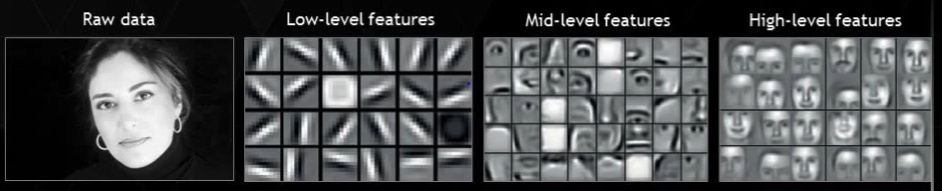
\includegraphics[width = 0.8\textwidth]{Images/deepConcept.png} 
\caption{Ejemplo de features \label{fig:deepconcept}}
\end{figure}

\subsection{Transfer Learning}
%- Explicar que es transfer learning 

En la práctica pocas personas entrenan una red profunda desde cero (con inicialización aleatoria), puesto a que éstas tienen unos requisitos bastante exigentes a la hora de ser entrenadas. 

Los mayores problemas que puedes encontrar son: 
\begin{enumerate}
\item A causa de la gran cantidad de parámetros a entrenar que tiene una red profunda necesitas un \textbf{conjunto de datos de gran tamaño}.
\item El \textbf{coste computacional} de entrenar la red, determinado por el número de parámetros, que en el caso de redes convolucionales  profundas pueden ser del orden de cientos de miles. 
\item La búsqueda de \textbf{hiper-parámetros} (valores de los que depende el modelo) óptimos. \par

La forma de obtener los hiper-parámetros es, entrenar la red para cada uno de los hiper-parámetros que hayamos considerado y, utilizando una partición de validación (o el método de \textit{cross-validation}) comparar los distintos resultados.  \par

Ésto incrementa los problemas \textit{1}, al necesitar una partición de validación necesitaremos más datos, y \textit{2}, el coste computacional se multiplica por cada vez que haya que entrenar la red, que puede ser varias veces por cada hiper-parámetro que tengamos.
\end{enumerate}\par
Por tanto, es común pre-entrenar una red convolucional en un conjunto de datos significativamente grande y usar la red convolucional como inicialización o como extractor fijo de características de la tarea de interés (como vemos en \cite{he2016deep}). 
\begin{definition}
Llamaremos \textbf{transfer learning} al campo de estudio que reutiliza el lenguaje de representación de un problema (que llamaremos problema origen o \textit{Source}) para resolver otro (que llamaremos objetivo o \textit{Target}). 

A la hora de utilizar \textbf{transfer learning} tenemos dos componentes base:  Un dominio $\mathcal{D}$ definido por un conjunto de instancias de datos con una distribución de probabilidades y una tarea $\mathcal{T}$, definida a partir de un conjunto de clases y una función objetivo.

Para un problema de \textit{transfer learning} usaremos la notación(introducida en \cite{pan2010survey}): 
\begin{itemize}
\item Problema origen: $(\mathcal{T_S},\mathcal{D_S})$
\item Problema objetivo: $(\mathcal{T_T},\mathcal{D_T})$
\end{itemize}

\end{definition}

Los dos casos más comunes de transfer learning son: 

\begin{itemize}
\item \textbf{Fine-tuning}(\cite{yosinski2014transferable}): La primera estrategia consiste en inicializar los datos desde un estado no aleatorio (tomando los pesos ya entrenados), y a continuación, entrenar la red sobre estos datos. 
De esta manera puedes reducir significativamente el conjunto de datos necesario para entrenarla, sin embargo, sigue necesitando tiempo para optimizar los múltiples hiper-parámetros involucrados en el proceso y una cantidad significativa de recursos computacionales. 
%En el caso de redes convolucionales esto se debe a que las primeras capas tienden a ser bastante generales.


\item \textbf{Feature Extraction}(\cite{pan2010survey}) Consiste en procesar un conjunto de datos a través de una red neuronal ya entrenada y extraer valores de activación para que puedan ser utilizados por otro mecanismo de aprendizaje. Este método es aplicable a conjuntos de datos de cualquier tamaño(\cite{azizpour2016factors}, \cite{sharif2014cnn} ), puesto que cada dato es procesado independientemente. Además tiene un menor coste computacional, ya que no tiene que entrenar la red y no requiere la optimización de hiper-parámetros. Por estos motivos las aplicaciones de \textit{transfer learning for feature extraction} están limitadas solo a las  capacidades de los métodos que utilices encima de la representación profunda obtenida. 


\end{itemize}

En nuestro caso nos centraremos en un tipo concreto de \textit{transfer learning for features extraction} \cite{behaviourcnn}, que explicaremos más adelante en la sección \ref{sec:fne}. 




\newpage

\section{Trabajo Relacionado}
\label{sec:trabajorelacionado}
\subsection{Full-Network embedding} \label{sec:fne}

En esta sección explicaré el \textit{full-network embedding} presentado en \cite{fne}.

En general en \textit{transfer learning for feature extraction} es común tomar los valores de activación de una sola capa cercana a la salida, como podemos ver en la figura \ref{fig:base}, donde el proceso de \textit{feature extraction} solo se hace en las últimas capas, \textit{fully-connected}, mientras que las capas convolucionales(todas las anteriores) permanecen intactas. El resto de capas se descartan por 
"ser poco probable que contengan una representación mejor"\cite{onlylastlayers}, sin embargo es conocido que todas las capas de una red profunda pueden contribuir a caracterizar los datos de diferentes maneras. Esto implica que la representación más versátil y rica que puede ser generada por un proceso de \textit{features extraction} debe incluir todas las capas de la red,es decir, debe definir un \textit{full-network embedding}. 
\begin{figure}[H]
\centering
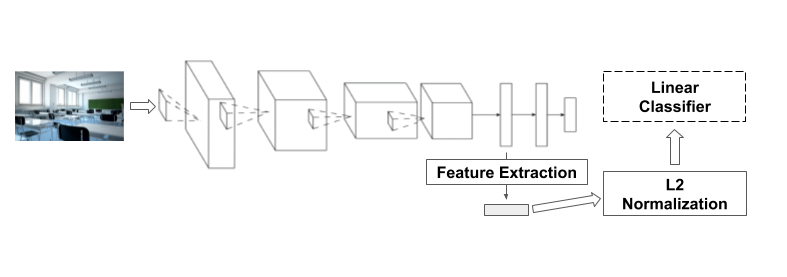
\includegraphics[width = 0.8\textwidth]{Images/basecrop.png} 
\caption{Estructura básica que se suele utilizar en \textit{feature extraction}
\label{fig:base}}
\end{figure}
Dado un conjunto de datos \textit{t1}, queremos representarlo en el lenguaje aprendido para una tarea \textit{t0}. Para ello el \textit{full-network embedding} se divide en 4 pasos: 
\begin{itemize}
\item El primer paso es hacer un \textbf{forward pass} de cada instancia de datos de \textit{t1} a través del modelo entrenado en \textit{t0}, guardando todos los valores de activación de cada capa de la red, (tanto las convolucionales como las \textit{fully-connected}). 

\item El segundo paso consiste en un \textbf{spatial average pooling} en los filtros convolucionales. Como se ha explicado en el capítulo sobre redes convolucionales, un filtro convolucional genera varias activaciones para una entrada, para darle la capacidad de obtener información espacial.  El objetivo de este paso es obtener un solo valor de activación para cada filtro, evitando así un aumento de la dimensionalidad. Los valores resultantes se concatenan a los de las capas \textit{fully-connected} en un solo vector, para generar el \textit{embedding} completo.

\item El tercer paso es una \textbf{estandarización de características}. Puesto a que los valores del \textit{embedding} provienen de distintos tipos de neuronas en distintos puntos de la red, la distribución de las activaciones pueden variar mucho y si se concatenasen todas algunas dominarían sobre las otras. \par
El valor estandarizado de cada categoría se obtiene calculando la media y la desviación típica del conjunto de datos de entrenamiento, es decir, que se estandariza según el contexto de la feature en todo el conjunto de datos. De esta forma se pueden integrar los distintos valores en el \textit{embedding}. 

\begin{figure}

\centering
\begin{tikzpicture}

\begin{axis}[no markers, domain=0:10, samples=100,
axis lines*=left, xlabel=, ylabel=,
height=6cm, width=10cm,
xticklabels={ , , -1 , $ft^-$ , 0 , $ft^+$ , 1},
ytick=\empty,
enlargelimits=false, clip=false, axis on top,
grid = major]
\addplot [fill=cyan!20, draw=none, domain=-1:1] {gauss(0,1)} \closedcycle;
\addplot [fill=blue!20, draw=none, domain=-3:-1] {gauss(0,1)} \closedcycle;
\addplot [fill=blue!20, draw=none, domain=1:3] {gauss(0,1)} \closedcycle;
\end{axis}
\end{tikzpicture}
\caption{
\label{fig:caracterization}}
\end{figure}

\item Finalmente se aplica una \textbf{discretización de características} para evitar problemas al intentar explorar un espacio de dimensión tan grande(una sola capa convolucional puede llegar a tener del orden de 100,000,000 parámetros, por ejemplo \cite{cnnexample}). Ésta discretización consiste en tomar unos límites que dependen de los datos, $ft^-$ y $ft^+$ y reemplazar los valores que tienen un valor atípicamente bajo (todos los valores $x < ft^-$) por un -1, los que tienen un valor típico (todos los valores $ ft^- < x < ft^+$) por un 0 y los que tienen un valor atípicamente alto (todos los valores $ ft^+ < x$) por un 1, como podemos ver en la representación gráfica \ref{fig:caracterization}. 

Para encontrar los límites, los autores se basan en \cite{behaviourcnn}, donde dan una visión estadística sobre como evaluar la importancia de las diferentes características de una red convolucional comparando las activaciones para una clase concreta respecto al resto de clases del conjunto de datos. De esta forma los autores de \cite{behaviourcnn} separan las características en tres conjuntos: \textit{característico por presencia}, \textit{no característico} y \textit{característico por ausencia}.
\end{itemize}

Un ejemplo de la separación comentada en la \textit{discretización de características} sería: si tenemos como datos objetivo un conjunto de coches tendremos que las features que se activen con las ruedas no serán representativas, puesto a que todos los coches tienen, las categorías que se activen con el techo de un coche serán representativas por ausencia para clasificar descapotables mientras que las que se activen para la capota serán representativas por presencia.


En la figura \ref{fig:fnediagram} podemos ver un diagrama de como se desarrollarían los diferentes pasos. Nótese la diferencia con la figura \ref{fig:base}. Mientras que en la figura \ref{fig:base} solo se modificaban las capas finales, en esta  se modifican también las convolucionales, dando lugar al \textit{full-network embedding} explicado.

\begin{figure}[h]
\label{fig:fne}
\centering
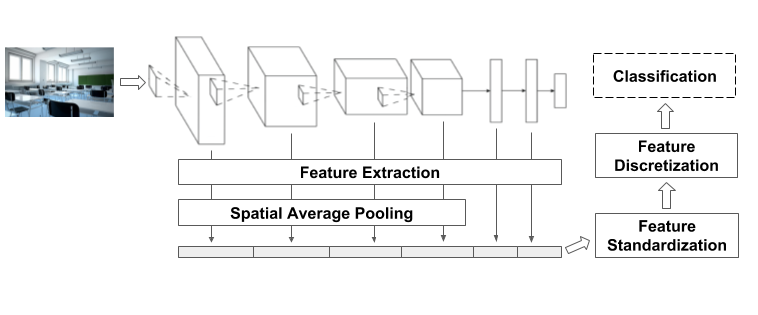
\includegraphics[width = 0.8\textwidth]{Images/cropfne.png} 
\caption{Estructura del \textit{full-network embedding}\label{fig:fnediagram}}
\end{figure}




\subsection{Wordnet}

\textbf{Wordnet} es una base de datos que contiene nombres, verbos, adjetivos y adverbios en conjuntos de sinónimos (que llamaremos \textit{synsets}). Los synsets están conectados entre ellos por medio de relaciones conceptuales, semánticas y léxicas. Utilizando los \textit{synsets} y sus relaciones, se puede generar un grafo que puede ser utilizado para distintos objetivos, como lingüística computacional y procesamiento del lenguaje natural. 

En concreto utilizaremos las relaciones de: 
\begin{itemize}

\item \textbf{Sinonimia} : dos palabras son sinónimos si tienen el mismo significado (ej, pelo y cabello, figura \ref{fig:sinonimos}).
\item \textbf{Hiponimia}: una palabra es hipónimo de otra si su significado es más específico que el de ésta (ej, mamífero es hipónimo de ser vivo, figura \ref{fig:hiponimos}). 
\item \textbf{Hipernimia}: una palabra es hiperónimo de otra si su significado es menos específico que el de ésta (ej, perro es hiperónimo de dálmata, figura \ref{fig:hiperonimos}). 
 
\end{itemize}


\begin{figure}[ht] 
	\centering
	\begin{subfigure}[b]{0.3\textwidth}
	\begin{tikzpicture}[
    grow=right,
    level 1/.style={sibling distance=3.5cm,level distance=3cm},
    edge from parent/.style={<->, draw, >=latex},
    edge from parent path={(\tikzparentnode.east) -- (\tikzchildnode.west)},
    punkt/.style={rectangle, rounded corners, shade, top color=blue!20, bottom color=blue!20, draw=blue!40!black!60, very
    thick }
    ]

\node[punkt] {Pelo}
    %Lower part lv1
    %Upper part, lv1
    child {
        node[punkt] {Cabello}
    };
\end{tikzpicture}
		\caption{Ejemplo de Sinónimos \label{fig:sinonimos}}
	\end{subfigure}
	\begin{subfigure}[b]{0.3\textwidth}
		\begin{tikzpicture}[sibling distance=10em,
  every node/.style = {shape=rectangle, rounded corners,
    draw, align=center,
    top color=blue!20, bottom color=blue!20},
    edge from parent/.style={draw,-latex}
    ]
  \node {Ser Vivo}
  	child{ node {Mamífero}
    	child{ node {Perro}}
    	child{node {Gato}}
    };
\end{tikzpicture}
		\caption{Ejemplo de Hipónimos \label{fig:hiponimos}}
	\end{subfigure}
	\begin{subfigure}[b]{0.3\textwidth}
		\begin{tikzpicture}[sibling distance=10em,
  every node/.style = {shape=rectangle, rounded corners,
    draw, align=center,
    top color=blue!20, bottom color=blue!20},
    edge from parent/.style={<-, draw,>=latex}
    ]
  \node {Perro}
    	child{node {Dálmata}}
    	child{node {Cachorro}
    	};
\end{tikzpicture}
		\caption{Ejemplo de Hiperónimos \label{fig:hiperonimos}}
	\end{subfigure}    
	\caption{}   
\end{figure}

%
%\begin{figure}[H]
%\centering
%
%\begin{tikzpicture}[sibling distance=10em,
%  every node/.style = {shape=rectangle, rounded corners,
%    draw, align=center,
%    top color=blue!20, bottom color=blue!20},
%    edge from parent/.style={draw,-latex}
%    ]
%  \node {Ser Vivo}
%  	child{ node {Mamífero}
%    	child{ node {Perro}}
%    	child{node {Gato}}
%    };
%\end{tikzpicture}
%\caption{Ejemplo de hipónimos}
%\end{figure}

\subsection{Imagenet}

\textbf{Imagenet} es una base de datos de imágenes organizada utilizando la jerarquía de \textit{wordnet}. Su principal objetivo es dotar a los investigadores en campos relacionados con visión artificial de una base de datos a gran escala con la que poder trabajar. Actualmente consta de 14,197,122 imágenes y  21,841 \textit{synsets} indexados.  

Para el full-network embedding utilizaron el subconjunto correspondiente al reto de \textit{imagenet} de 2012 de reconocimiento de imágenes. 

Éste consta de:
\begin{itemize}
\item Un conjunto de datos de entrenamiento de 1.2 millones de muestras y 1,000 categorías diferentes.
\item Un conjunto de datos de validación de 50,000 muestras y 1,000 categorías. 
\end{itemize}

Entre las posibles categorías podemos encontrar \textit{synsets} de diferentes niveles de especificación, por ejemplo tenemos las categorías: perro, dálmata, pastor alemán... 

\newpage
\section{Enfoque}
\label{sec:enfoque}
En nuestro caso estudiaremos un \textit{full-network embedding} obtenido a partir de la tarea origen  $(\mathcal{T_S} = $Clasificación de imágenes$,\mathcal{D_S} =$ 1.2 M imágenes de imagenet con sus correspondientes clases$ )$ y una tarea de destino $(\mathcal{T_T} = $Clasificación de imágenes$,\mathcal{D_T} =$ 50,000 imágenes de imagenet con sus correspondientes clases$ )$. Es decir, partiendo de una red convolucional entrenada con todo el conjunto de datos de entrenamiento de imagenet, hemos generado un lenguaje de representación para el conjunto de datos de validación de imagenet. Lo que resulta en el \textit{full-network embedding} con el que trabajaremos. 

El \textit{full-network embedding} consiste en una matriz de tamaño 50,000 muestras por 12,416 características, como observamos en la figura \ref{fig:featuresperlayer}, cuyos valores están en $\{-1,0,1\}$. Para cada muestra también tenemos su correspondiente clasificación (un valor entre 0 y 999 que representa la clase de imagenet con la que fue clasificado).

Es importante remarcar el significado de las diferentes categorías.
\begin{itemize}
\item Si el valor para una imagen concreta es 1 significa que esta es representativa por presencia. Es decir, que dentro del contexto del conjunto de datos \textit{Target}, es una \textit{feature} característica de una clase concreta.
\item Si el valor para una imagen concreta es 0 significa que esa característica no es representativa.
\item Si el valor para una imagen concreta es -1 significa que es representativa por ausencia. 
\end{itemize}

Hemos de tener en cuenta que estas definiciones son con respecto a $\mathcal{D_T}$, es decir, respecto al nuevo espacio de representación.  

Las características están ordenadas en capas de la siguiente manera: 
\begin{figure}[H]
\label{}
\centering
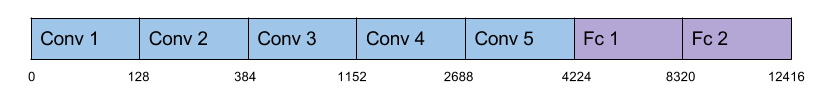
\includegraphics[width = 0.8\textwidth]{Images/croplayer.png} 
\caption{La disposición de las características por capas \label{fig:featuresperlayer}}
\end{figure}
%'fc6': [4224, 8320],  # 14
%			'fc7': [8320, 12416],  # 15
%			'conv1': [0, 128],  # 16
%			'conv2': [128, 384],  # 17
%			'conv3': [384, 1152],  # 18
%			'conv4': [1152, 2688],  # 19
%			'conv5': [2688, 4224],  # 20

%Además tomamos 3 embeddings diferentes:
%\begin{itemize}
%\item El básico con los límites en $ft^- = -0.25$ y $ft^+ = +0.25$ 
%\item Un embedding más restrictivo con los límites en $ft^- = -0.19$ y $ft^+ = +0.19$ 
%\item Un embedding menos restrictivo con los límites en $ft^+ = -0.31$ y $ft^+ = +0.31$ 
%\end{itemize}

Finalmente, de todos los \textit{synsets} posibles tomamos dos subconjuntos diferentes: 

\begin{figure}[H]
\centering
\begin{subfigure}{.5\textwidth}
  \centering
  %\includegraphics[width=.4\linewidth]{image1}
\begin{tikzpicture}[sibling distance=10em,
  every node/.style = {shape=rectangle, rounded corners,
    draw, align=center,
    top color=cyan!20, bottom color=cyan!20},
    edge from parent/.style={draw,-latex}
    ]
  \node {Ser Vivo}
  	child{ node {Mamífero}
    	child{ node {Perro}
			child{node {Perro de caza}    	
    		}
    	}
    };
\end{tikzpicture}
  \caption{Seres vivos}
  \label{fig:sub1}
\end{subfigure}%
\begin{subfigure}{.5\textwidth}
  \centering
  \begin{tikzpicture}[sibling distance=10em,
  every node/.style = {shape=rectangle, rounded corners,
    draw, align=center,
    top color=red!20, bottom color=red!20},
    edge from parent/.style={draw,-latex}
    ]
  \node {Artefacto}
  	child{ node {Instrumento}
    	child{ node {Transporte}
			child{node {Vehículo}    	
    		}
    	}
    };
\end{tikzpicture}
  \caption{Objetos}
  \label{fig:sub2}
\end{subfigure}
\caption{Conjuntos de synsets que estudiaremos \label{fig:synsets}}

\end{figure}

Hemos tomado estos dos conjuntos por estar distribuidos de una forma bastante uniforme entre las clases, como veremos en el capítulo \ref{se:stats}, y por ser de dos ''ramas'' lo más diferentes posibles,además están en sitios parecidos respecto a la jerarquía global, y por tanto representan niveles de abstracción parecidos. 

 
\subsection{Objetivos}
Partiendo de los datos comentados y del trabajo publicado en \cite{fne} tomamos varios \textbf{objetivos} a partir de los que desarrollar el trabajo.

\begin{itemize}
\item Analizar el \textit{embedding} dado y el comportamiento de las \textit{features} en las distintas capas. Para ello se realizará un estudio estadístico inicial de la matriz de \textit{embeddings}. De este estudio se analizarán los diferentes puntos de interés, y finalmente se hará un estudio más detallado de estos.  
\item Analizar si hay alguna relación entre los \textit{embeddings} de las diferentes clases y \textit{synsets} relacionados con ellas (sus hipónimos e hipérnimos). Para ello se realizarán las estadísticas del comportamiento de los \textit{synsets} de la figura \ref{fig:synsets} con respecto a la matriz de \textit{embeddings}, con intención de profundizar en los puntos de interés que se encuentren. 
\end{itemize}

\subsection{Estadísticas}\label{se:stats}
La finalidad de este capítulo es hacer un estudio inicial de los datos de los que se dispone, es decir, de los correspondientes al \textit{embedding} y a los \textit{synsets} que hemos tomado para el estudio. 

\subsubsection{Synsets}

Como comentamos en la sección anterior los \textit{synsets} que hemos tomado son \ref{fig:synsets}. 
El criterio que hemos utilizado para decidir que una clase de \textit{Imagenet} pertenece a un \textit{synset} es que sea hipónimo de esta, por tanto es coherente que los \textit{synsets} más generales tengan más imágenes. 
 
Además, ambas familias (la de seres vivos y objetos), se distribuyen de forma parecida (cada \textit{synset} hijo tiene aproximadamente la mitad de imágenes que su \textit{synset} padre), como podemos ver en la figura \ref{fig:totalsynsets}. Elegimos dos familias de \textit{synsets} que cumplieran esto para que al comparar los resultados se distorsionaran lo menos posible por la cantidad de imágenes pertenecientes a ellas.

\begin{figure}[H] 
	\centering
	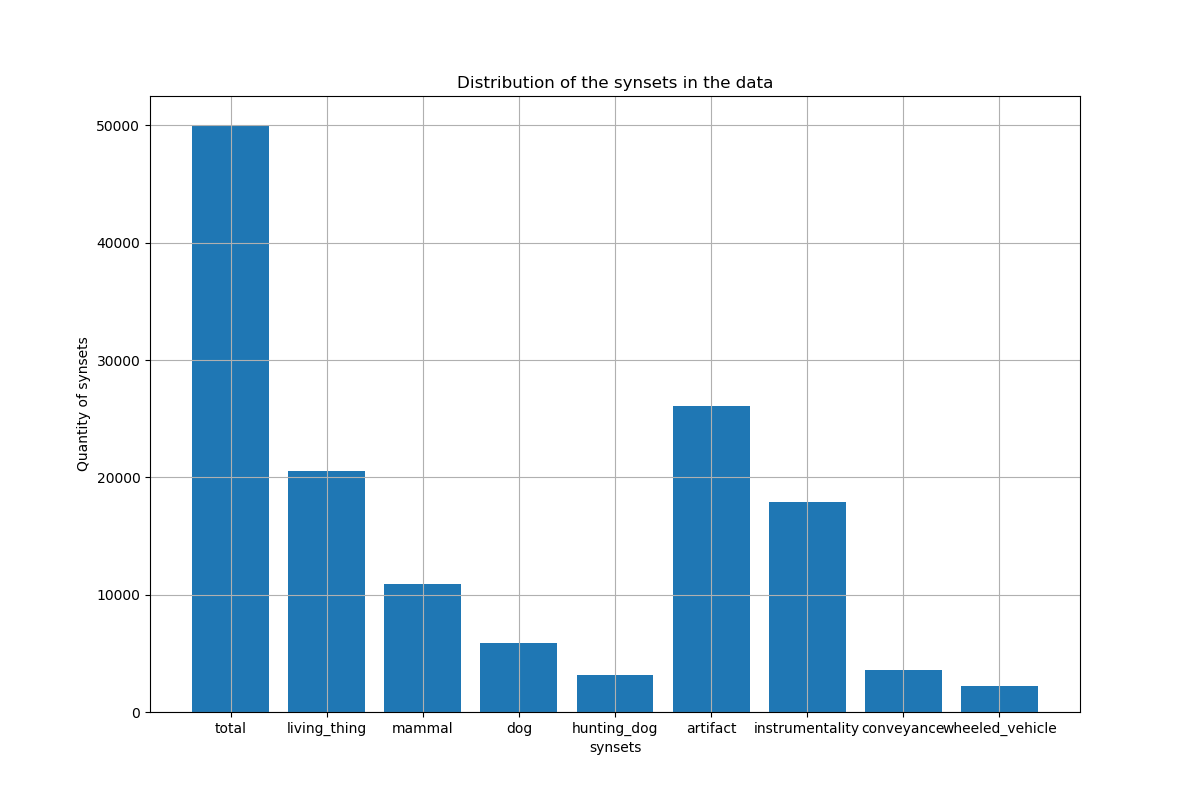
\includegraphics[width=0.8\textwidth] {Images/plots/25/distribution_of_synsets_bar.png}
	\caption{ Distribución de los \textit{synsets} en el embedding
	\label{fig:totalsynsets}}
\end{figure}


\subsubsection{Visión de conjunto del Embedding e Hipótesis iniciales}
Primero de todo estudiaremos las estadísticas generales del \textit{embeddings}.
Empezando con la cantidad de elementos de cada categoría. 

\begin{figure}[ht] 
	\centering
	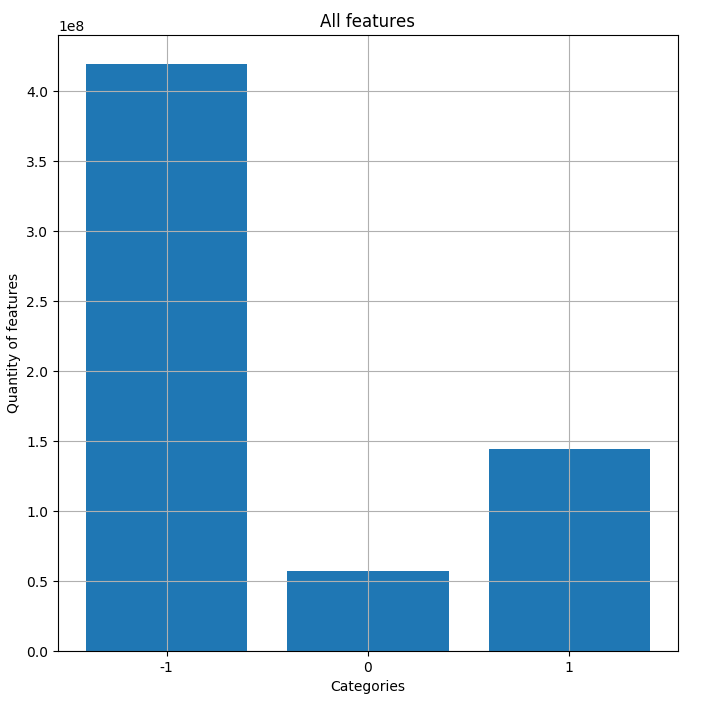
\includegraphics[width=0.4\textwidth] {Images/plots/25/quantity_of_features_bar.png}
	\caption{ Cantidad de \textit{features} de cada categoría
	\label{fig:totalfeatures}}


\end{figure}

En la figura \ref{fig:totalfeatures} vemos la cantidad de \textit{features} de cada categoría. Podemos observar que la cantidad total de -1 es significativamente mayor, esta distribución se conserva (en general) para los distintos \textit{synsets}, independientemente de lo específicos que sean. Teniendo en cuenta que al hacer \textit{transfer learning} se suele pasar de un conjunto de datos más general a uno más específico que haya más \textit{features} características por ausencia es coherente. Más adelante veremos también como se distribuyen las categorías entre las diferentes capas del \textit{embedding}. 


Observamos también como se distribuyen las \textit{features} respecto al conjunto de imágenes que tenemos. 

\begin{figure}[ht] 
	\centering
	\begin{subfigure}[b]{0.3\textwidth}
		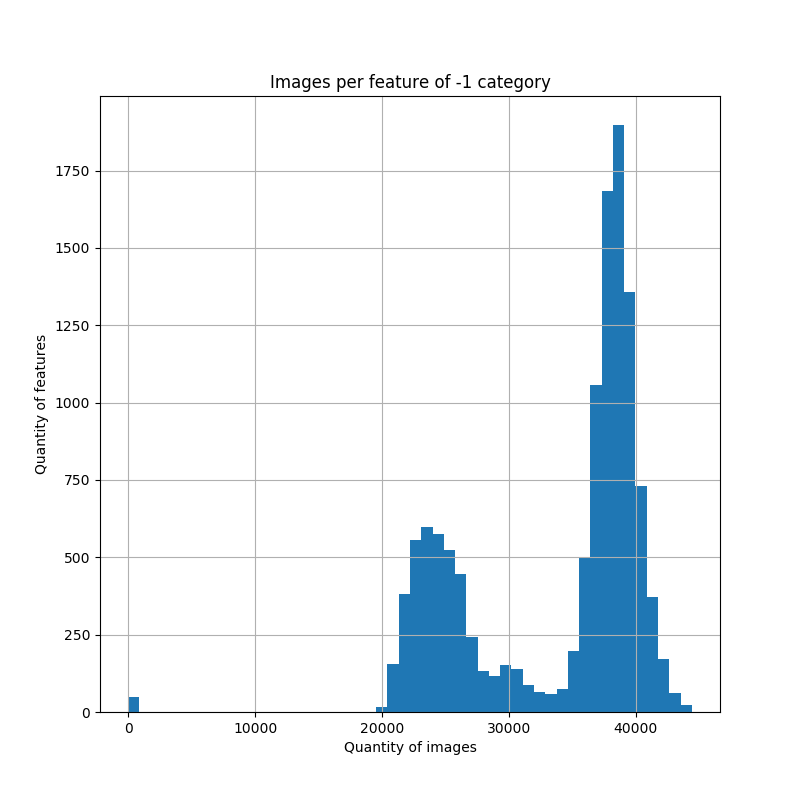
\includegraphics[width=\textwidth] {Images/plots/25/Images_per_feature_of_-1_category.png}
		\caption{Categoría -1}
	\end{subfigure}
	\begin{subfigure}[b]{0.3\textwidth}
		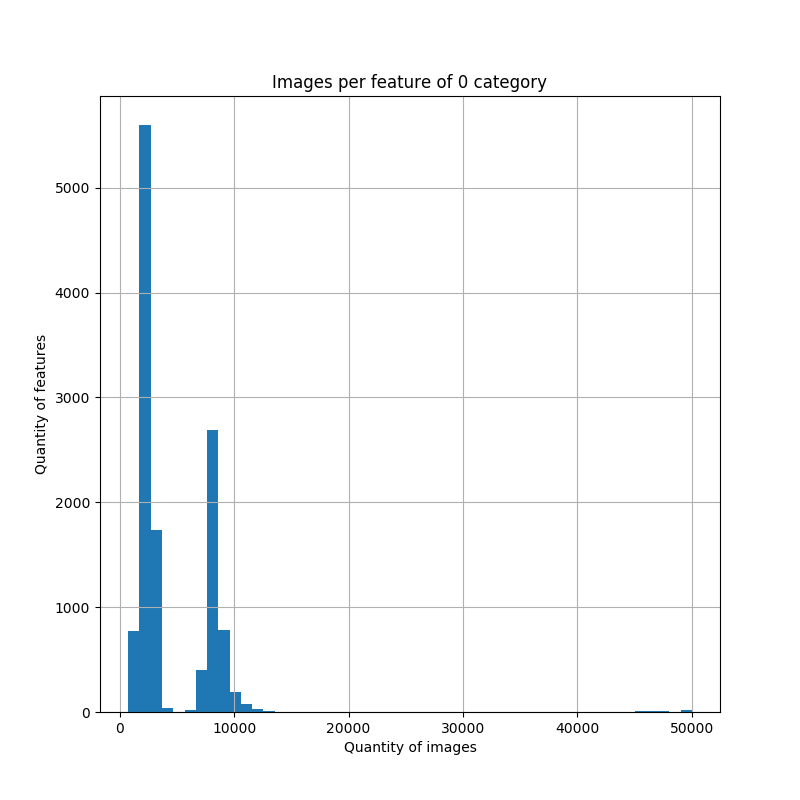
\includegraphics[width=\textwidth]  {Images/plots/25/Images_per_feature_of_0_category.png}
		\caption{Categoría 0}
	\end{subfigure}
	\begin{subfigure}[b]{0.3\textwidth}
		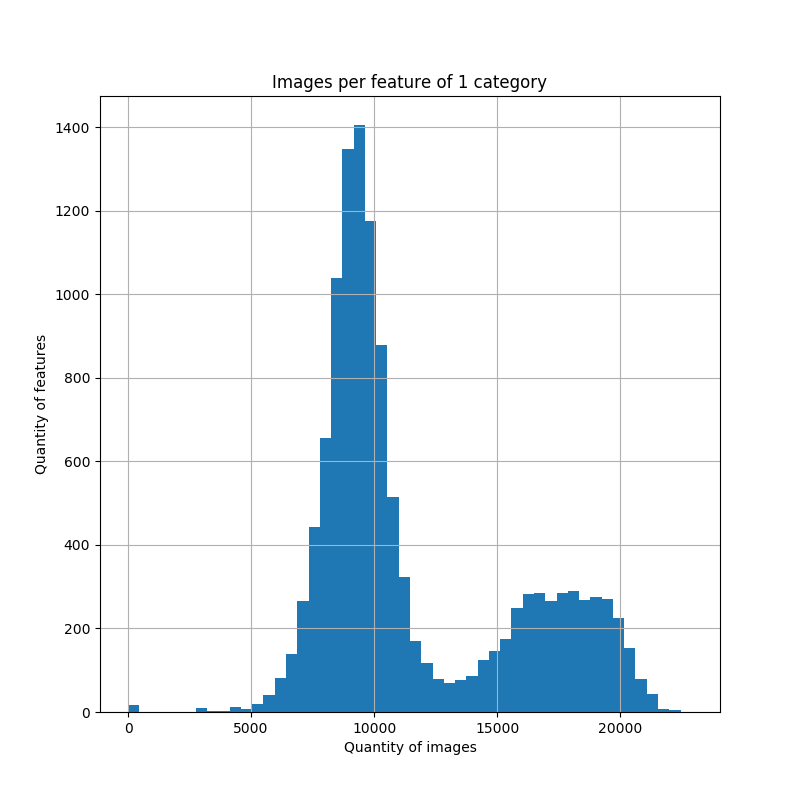
\includegraphics[width=\textwidth]  {Images/plots/25/Images_per_feature_of_1_category.png}
		\caption{Categoría 1}
	\end{subfigure}       
	\caption{Imágenes por categoría \label{fig:imagesperfeature}}
\end{figure}

En la figura \ref{fig:imagesperfeature} tenemos la distribución de las imágenes por categoría, es decir cuantas imágenes tienen una cierta cantidad de \textit{features}. La idea de generar esta gráfica era ver si podíamos encontrar alguna distribución concreta o patrón. %En las tres categorías se ven dos distribuciones bien diferenciadas, lo que hace plantearse si depende de los dos tipos de capas diferentes del \textit{embedding} (las convolucionales y las completas).

Al estudiar la matriz de embeddings nos planteamos las siguientes hipótesis: 
\begin{enumerate}
\item \label{h1} Las características se distribuyen de diferente manera en las capas convolucionales y los completos. Esta hipótesis proviene de la gráfica \ref{fig:imagesperfeature}, donde 
en las tres categorías se ven dos distribuciones bien diferenciadas. Otro motivo para pensar que las características se distribuyen de forma diferente es que las capas \textit{fully-connected} tienen más \textit{features} que las convolucionales.
\item \label{h2} Cuanto más concreto es un \textit{synset}, debería haber más features representativas, tanto por ausencia como por presencia.
\item \label{h3} Cuanto más profundo es el layer, debería haber más features representativas, tanto por ausencia como por presencia. Esta hipótesis viene de que en una red convolucional cuanto más profunda es una capa más concretas suelen ser las features con las que se activa, como vimos en la figura \ref{fig:deepconcept}.
\item \label{h4} Se puede ver una relación entre los embeddings de synsets hipónimos. La idea sería que dada una imagen perteneciente a un \textit{synset}, compartiría \textit{features} características con sus hipónimos.
\end{enumerate}


\newpage
\section{Análisis}
\label{sec:analisis}
\subsection{De Wordnet al Full Network Embedding}
%En este apartado explicaré: 
%
%\begin{itemize}
%\item Las distribuciones de las imágenes por feature son diferentes para conv y fc, y mantienen la forma entre embeddings.
%\item Las distribuciones de las imágenes por feature por layer por synset se conservan. 
%\item Explicar los resultados de las matrices de cambio. 
%\item Cuanto más concreto es el synset mayor proporción de 1. 
%\end{itemize}

En este apartado explicaré el estudio hecho para intentar aceptar o revocar las hipótesis comentadas. Empezaré con la distribución por tipo de capa en el \textit{embedding} general, para luego concretar estudiando el comportamiento por capa. Finalmente explicaré los descubrimientos relacionados con los \textit{synsets}. 
\subsubsection{Distribución por tipo de capa}
Para comprobar si la hipótesis \ref{h1} es cierta calculamos las gráficas de la figura \ref{fig:imagesperfeature} distinguiendo entre las capas convlolucionales y \textit{fully-connected}, obteniendo las siguientes gráficas: 

\begin{figure}[ht] 
	\centering
	\begin{subfigure}[b]{0.3\textwidth}
		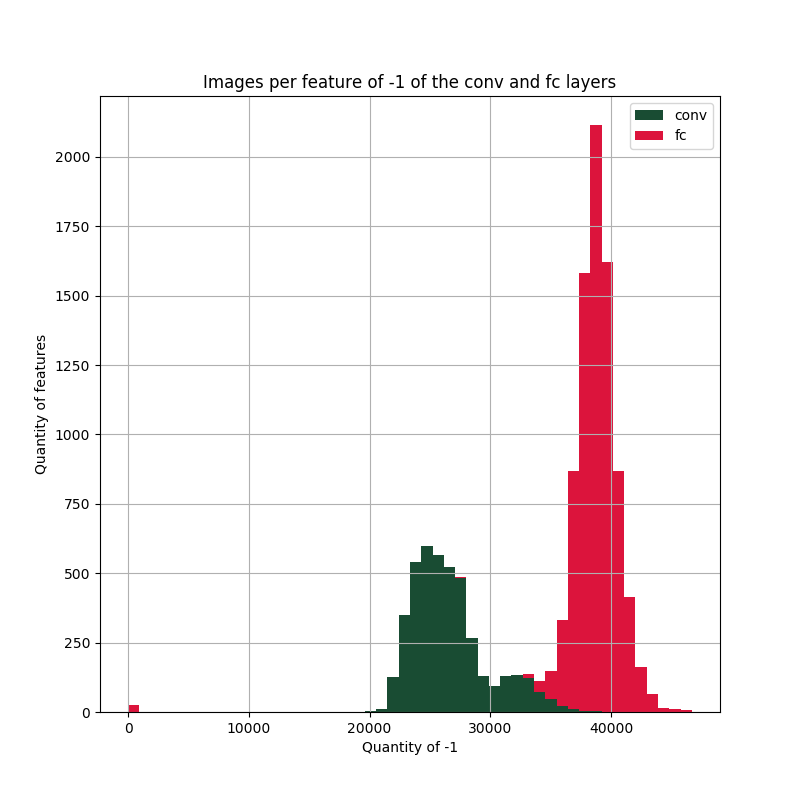
\includegraphics[width=\textwidth] {Images/plots/25/Images_per_feature_of_-1_category_all_layers.png}
		\caption{Categoría -1}
	\end{subfigure}
	\begin{subfigure}[b]{0.3\textwidth}
		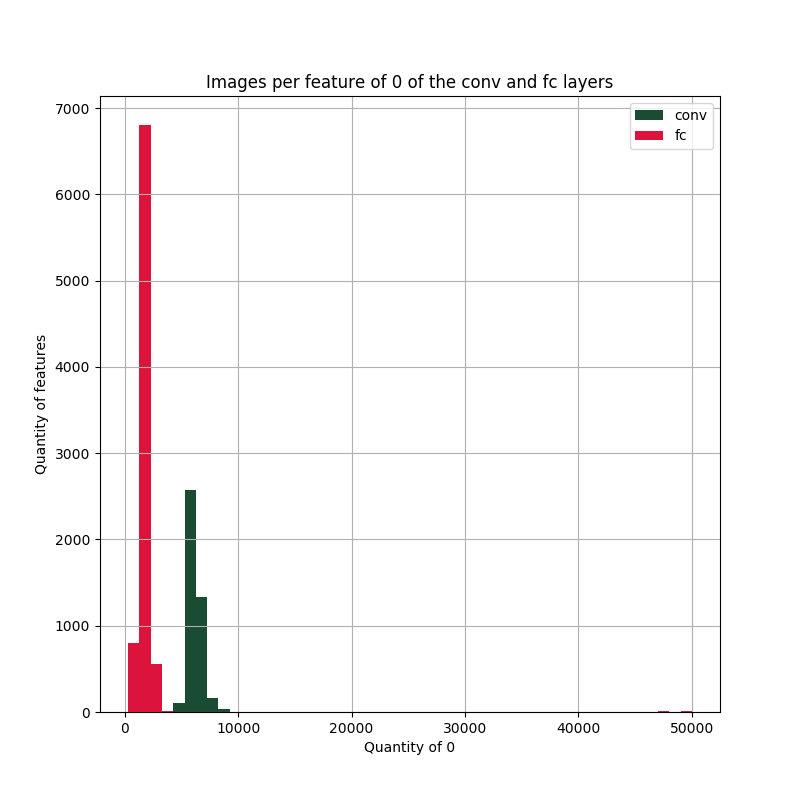
\includegraphics[width=\textwidth]  {Images/plots/25/Images_per_feature_of_0_category_all_layers.png}
		\caption{Categoría 0}
	\end{subfigure}
	\begin{subfigure}[b]{0.3\textwidth}
		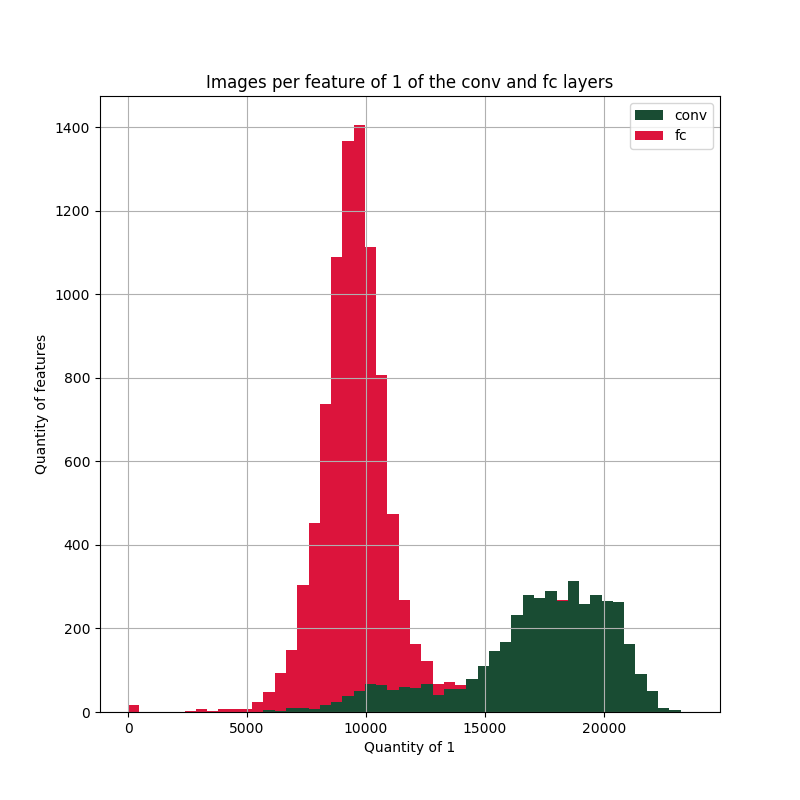
\includegraphics[width=\textwidth]  {Images/plots/25/Images_per_feature_of_1_category_all_layers.png}
		\caption{Categoría 1}
	\end{subfigure}       
	\caption{Imágenes por \textit{feature} \label{fig:imagesperfeature}}
\end{figure}

En ellas podemos ver claramente la distinción que suponíamos. Sobretodo para la categoría 0, hay una clara separación entre el comportamiento de los diferentes tipos de capa. En parte esto se debe a que hay más \textit{features} en las capas \textit{fully-connected}, por eso sus gráficas correspondientes son más altas, además en éstas podemos ver una menor variabilidad, que concuerda con el hecho de que solamente son 2 capas \textit{fully-connected}, contra las 5 convolucionales. También vemos que el grueso de las features características (tanto por presencia como por ausencia) se encuentran en las capas \textit{fully-connected}, cosa que concuerda con el hecho de que sean estas capas las que dan la clasificación final. 
 
\subsubsection{Comportamiento respecto a la profundidad}

Una vez comprobado que los dos tipos de capa se comportan diferente, vamos a estudiar en que nivel se diferencian y a que profundidad. De esta forma veremos si podemos aceptar o desmentir la hipótesis \ref{h3}. 

Para ello hemos calculado la cantidad de \textit{features} de cada tipo por capa respecto al \textit{embedding} total. Como podemos observar en la gráfica \ref{fig:totalfeaturesperlayer}. De esta forma se esperaba ver como se distribuyen las \textit{features} por cada capa.


\begin{figure}[ht] 
	\centering
	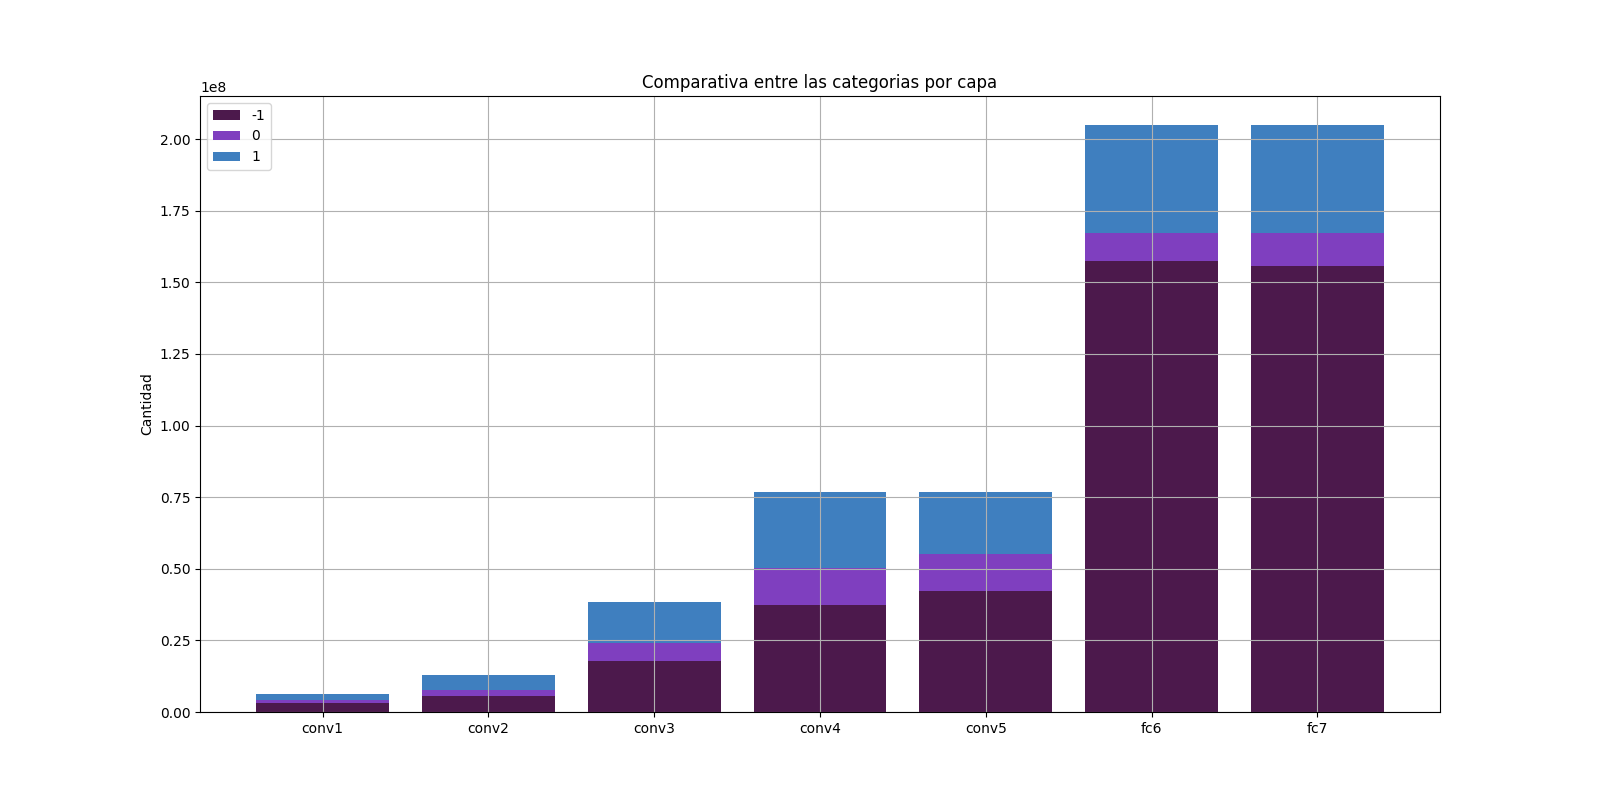
\includegraphics[width=0.9\textwidth] {Images/plots/25/Comparative_of_synsets_all.png}
	\caption{ Cantidad de \textit{features} de cada categoría por capa
	\label{fig:totalfeaturesperlayer}}
\end{figure}

En la gráfica esperábamos encontrar una mayor proporción de \textit{features} características por presencia en las capas finales, sin embargo podemos ver que la mayor proporción se encuentra en la cuarta capa convolucional. En esta gráfica podemos ver claramente que todas las capas, no solo las \textit{fully-connected} contienen información importante de cara a caracterizar el espacio de representación, al contrario de lo que sostienen en \cite{onlylastlayers}.

\subsubsection{Comportamiento de los synsets} \label{sec:synsets}

A la hora de estudiar los \textit{synsets} nos hemos topado con la dificultad de decidir el valor de una \textit{feature} para el conjunto de todas las muestras que pertenecen al \textit{synset}, puesto a que para diferentes muestras puede tener distintos valores, como podemos ver en el ejemplo de la figura \ref{fig:muestrasynsets}. 


\begin{figure}[h]
\begin{center}
\begin{tikzpicture}[mymatrixenv]

	\matrix (mtr) [matrix of nodes,column sep=-\pgflinewidth, row sep=-\pgflinewidth,  nodes={draw,
      minimum height=0.5cm,
      anchor=center,
      text width=0.5cm,
      align=center,
      inner sep=0pt
    }]
	{
		|[fill=blue!30]| 1 & |[fill=blue!30]| 1 & |[fill=blue!30]| -1 & |[fill=blue!30]| 1 & |[fill=blue!30]| 0 & |[fill=blue!30]| 0 & |[fill=blue!30]| -1\\
		0 & 0 & -1 & -1 & -1 & 0 & 0\\
		0 & 0 & 0 & 1 & -1 & -1 & 0\\
		|[fill=green!30]| 1 & |[fill=green!30]| 1 & |[fill=green!30]| -1 & |[fill=green!30]| 1 & |[fill=green!30]| -1 & |[fill=green!30]| 0 & |[fill=green!30]| 0\\
		0 & 0 & -1 & 1 & 0 & 0 & 0\\
		0 & -1 & 1 & 0 & 0 & 0 & 1\\
		|[fill=blue!30]| 1 & |[fill=blue!30]| 1 & |[fill=blue!30]| -1 & |[fill=blue!30]| -1 & |[fill=blue!30]| -1 & |[fill=blue!30]| 0 & |[fill=blue!30]| 0\\
		-1 & -1 & 0 & 0 & 0 & 0 & 0\\
	};

	\draw[very thick, blue] (mtr-1-1.north west) rectangle (mtr-1-7.south east);
	\draw[very thick, green] (mtr-4-1.north west) rectangle (mtr-4-7.south east);
	\draw[very thick, blue] (mtr-7-1.north west) rectangle (mtr-7-7.south east);
    \node[left=12pt of mtr-1-1] (left-1) {ser vivo};
    \node[left=12pt of mtr-7-1] (left-3) {ser vivo};
    \node[left=12pt of mtr-4-1] (left-2) {mamífero};
    
    \mymatrixbracetop{1}{7}{\textit{features}}
 \mymatrixbraceleft{1}{8}{muestras}


\end{tikzpicture}
\end{center}
\caption{Muestra de una sección del embedding.
\label{fig:muestrasynsets}
}
\end{figure}

Para solucionar este problema hemos decidido tomar dos enfoques diferentes, por un lado hemos tomado la sub-matriz correspondiente a cada \textit{synset}, por otro lado hemos tomado un vector representante para cada \textit{synset} a estudiar. 

\textbf{Sub-matriz:}

En este caso hemos tomado una matriz cuyas filas consisten en las muestras que pertenecen al \textit{synset} que queremos estudiar y cuyas columnas corresponden a las \textit{features}, como muestra el ejemplo de la figura \ref{fig:submatrix}.

\begin{figure}[H]
\begin{center}
%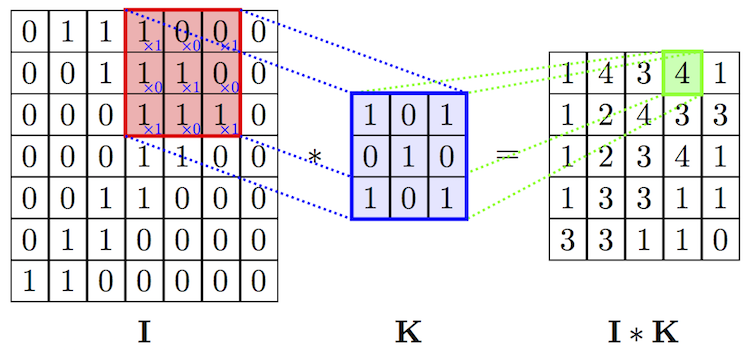
\includegraphics[width = 0.5\textwidth]{Images/convolve.png} 
\begin{tikzpicture}

	\matrix (mtr) [matrix of nodes,column sep=-\pgflinewidth, row sep=-\pgflinewidth,  nodes={draw,
      minimum height=0.5cm,
      anchor=center,
      text width=0.5cm,
      align=center,
      inner sep=0pt
    }]
	{
		|[fill=blue!30]| 1 & |[fill=blue!30]| -1 & |[fill=blue!30]| -1 & |[fill=blue!30]| 1 & |[fill=blue!30]| 0 & |[fill=blue!30]| 0 & |[fill=blue!30]| -1\\
		0 & 0 & -1 & -1 & -1 & 0 & 0\\
		0 & 0 & 0 & 1 & -1 & -1 & 0\\
		|[fill=green!30]| 0 & |[fill=green!30]| 1 & |[fill=green!30]| -1 & |[fill=green!30]| 1 & |[fill=green!30]| 1 & |[fill=green!30]| 0 & |[fill=green!30]| 0\\
		|[fill=blue!30]| 1 & |[fill=blue!30]| 1 & |[fill=blue!30]| -1 & |[fill=blue!30]| 0 & |[fill=blue!30]| -1 & |[fill=blue!30]| 0 & |[fill=blue!30]| 0\\
		0 & 0 & -1 & 1 & 0 & 0 & 0\\
		0 & -1 & 1 & 0 & 0 & 0 & 1\\
		|[fill=blue!30]| 1 & |[fill=blue!30]| 1 & |[fill=blue!30]| 1 & |[fill=blue!30]| -1 & |[fill=blue!30]| -1 & |[fill=blue!30]| 0 & |[fill=blue!30]| 0\\
		-1 & -1 & 0 & 0 & 0 & 0 & 0\\
	};

    \node [below= of mtr-7-4.south] (lm) {embedding};
    

	\matrix (K) [right=5em of mtr,matrix of nodes,row sep=-\pgflinewidth, nodes={draw,minimum height=0.5cm,
      anchor=center,
      text width=0.5cm,
      align=center,
      inner sep=0pt, fill=blue!30}]
	{
		1 & -1 & -1 &  1 &  0 & 0 & -1\\
		1 &  1 & -1 &  0 & -1 & 0 & 0\\
		1 &  1 &  1 & -1 & -1 & 0 & 0\\
	};
    \node [below= of K-2-4.south] (lk) {sub-matriz};

    \draw[very thick, blue] (K-1-1.north west) rectangle (K-3-7.south east);
	
	\draw[densely dotted, blue, thick] (mtr-1-1.north west) -- (K-1-1.north west);
	\draw[densely dotted, blue, thick] (mtr-1-1.south west) -- (K-1-1.south west);
	\draw[densely dotted, blue, thick] (mtr-1-7.north east) -- (K-1-7.north east);
	\draw[densely dotted, blue, thick] (mtr-1-7.south east) -- (K-1-7.south east);
	
	\draw[densely dotted, blue, thick] (mtr-5-1.north west) -- (K-2-1.north west);
	\draw[densely dotted, blue, thick] (mtr-5-1.south west) -- (K-2-1.south west);
	\draw[densely dotted, blue, thick] (mtr-5-7.north east) -- (K-2-7.north east);
	\draw[densely dotted, blue, thick] (mtr-5-7.south east) -- (K-2-7.south east);
	
    \draw[densely dotted, blue, thick] (mtr-8-1.north west) -- (K-3-1.north west);
	\draw[densely dotted, blue, thick] (mtr-8-1.south west) -- (K-3-1.south west);
	\draw[densely dotted, blue, thick] (mtr-8-7.north east) -- (K-3-7.north east);
	\draw[densely dotted, blue, thick] (mtr-8-7.south east) -- (K-3-7.south east);
\end{tikzpicture}
\end{center}
\caption{Ejemplo de una submatriz de un \textit{synset}.
\label{fig:submatrix}}
\end{figure}

Este enfoque nos da información general sobre el comportamiento de los distintos \textit{synsets} en el \textit{embedding}. 

Utilizando la sub-matriz asociada a cada uno de los \textit{synsets} hemos generado gráficas equivalentes a la de la figura \ref{fig:imagesperfeature}. En este caso, las distribuciones se mantienen bastante en los \textit{synsets} más generales, como podemos ver en la figura \ref{fig:imagesperfeatureliving}, mientras que en los menos generales se empiezan a distorsionar. Como podemos observar en la figura \ref{fig:imagesperfeaturewheel}.

\begin{figure}[ht] 
	\centering
	\begin{subfigure}[b]{0.3\textwidth}
		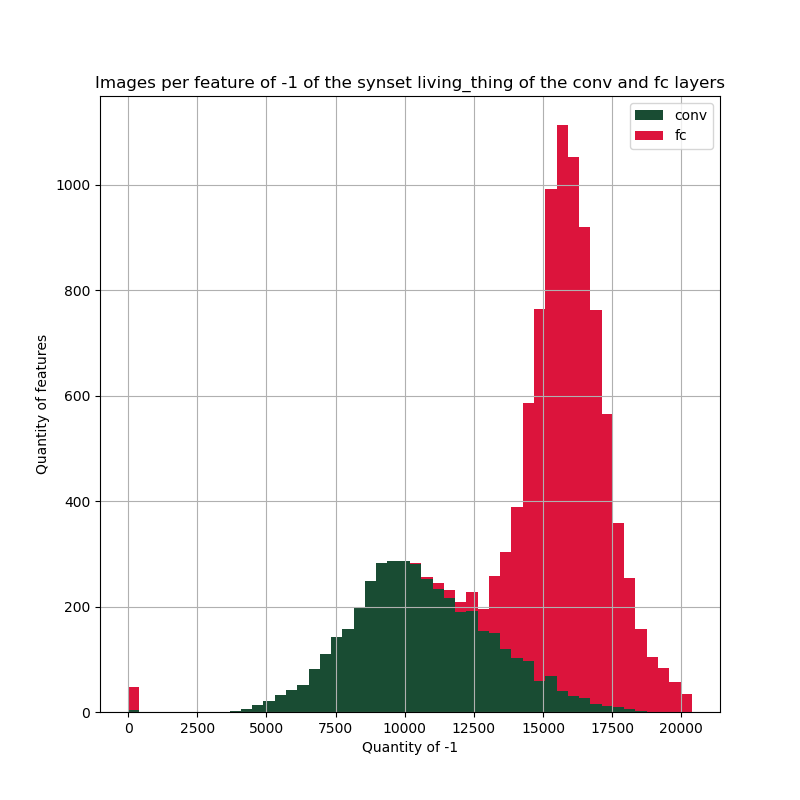
\includegraphics[width=\textwidth] {Images/plots/25/synsets/Images_per_feature_of_-1_category_living_thingall_layers.png}
		\caption{Categoría -1}
	\end{subfigure}
	\begin{subfigure}[b]{0.3\textwidth}
		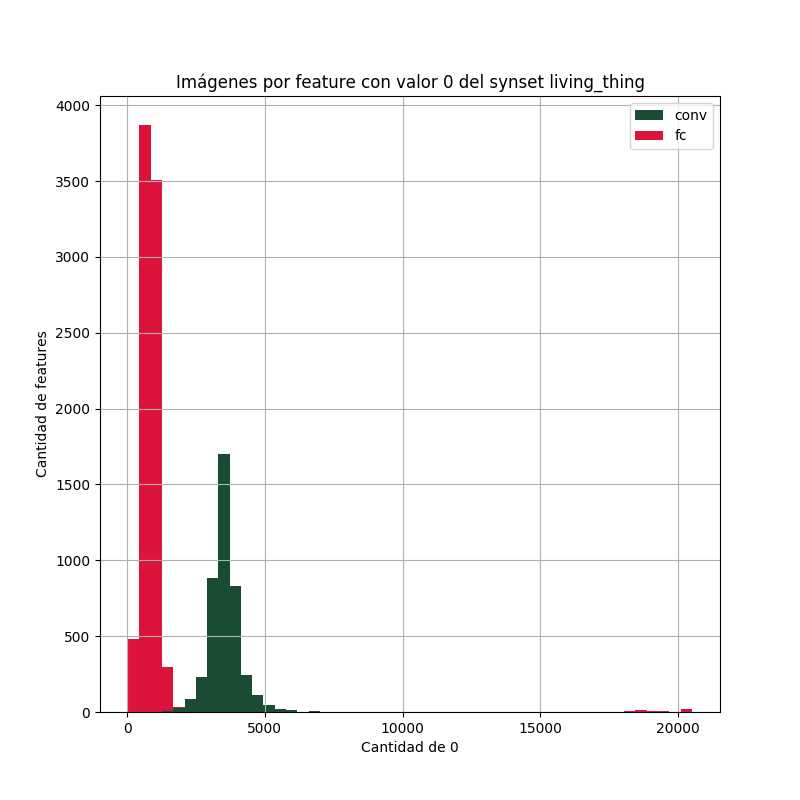
\includegraphics[width=\textwidth]  {Images/plots/25/synsets/Images_per_feature_of_0_category_living_thingall_layers.png}
		\caption{Categoría 0}
	\end{subfigure}
	\begin{subfigure}[b]{0.3\textwidth}
		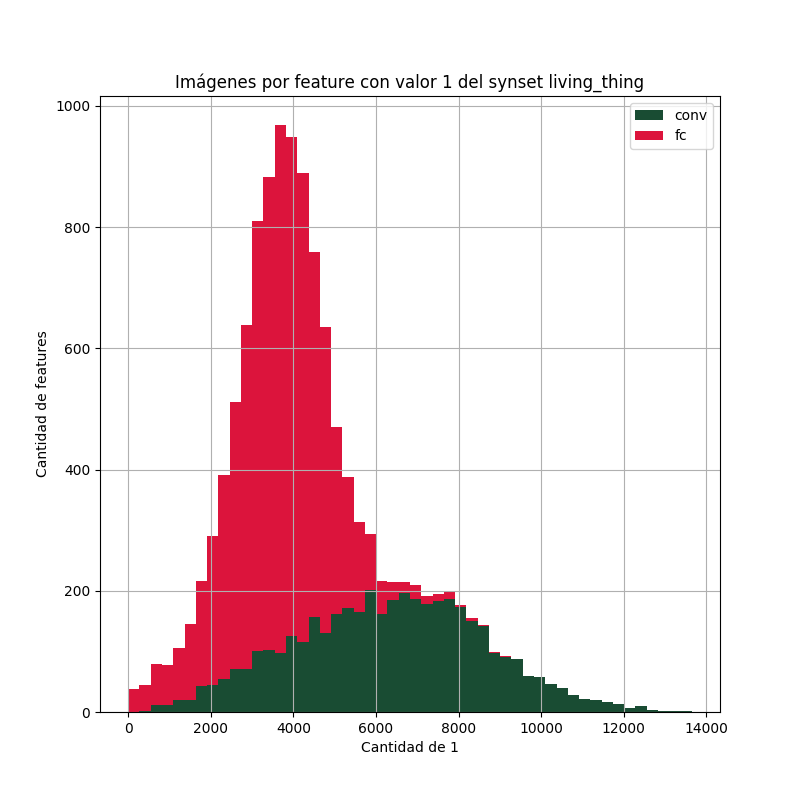
\includegraphics[width=\textwidth]  {Images/plots/25/synsets/Images_per_feature_of_1_category_living_thingall_layers.png}
		\caption{Categoría 1}
	\end{subfigure}       
	\caption{Imágenes por categoría del \textit{synset} seres vivos \label{fig:imagesperfeatureliving}}
\end{figure}

\begin{figure}[ht] 
	\centering
	\begin{subfigure}[b]{0.3\textwidth}
		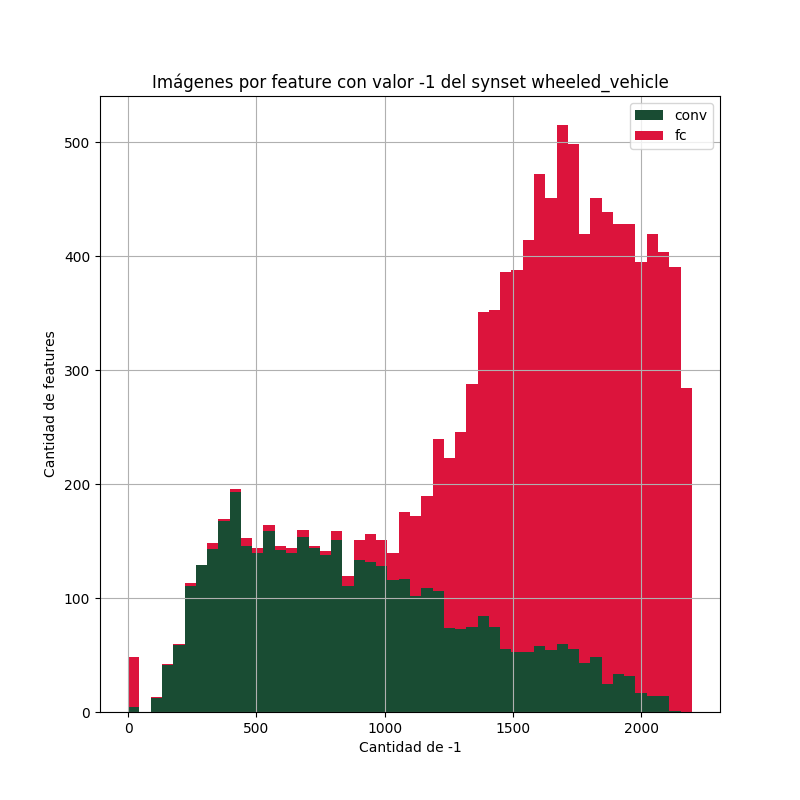
\includegraphics[width=\textwidth] {Images/plots/25/synsets/Images_per_feature_of_-1_category_wheeled_vehicleall_layers.png}
		\caption{Categoría -1}
	\end{subfigure}
	\begin{subfigure}[b]{0.3\textwidth}
		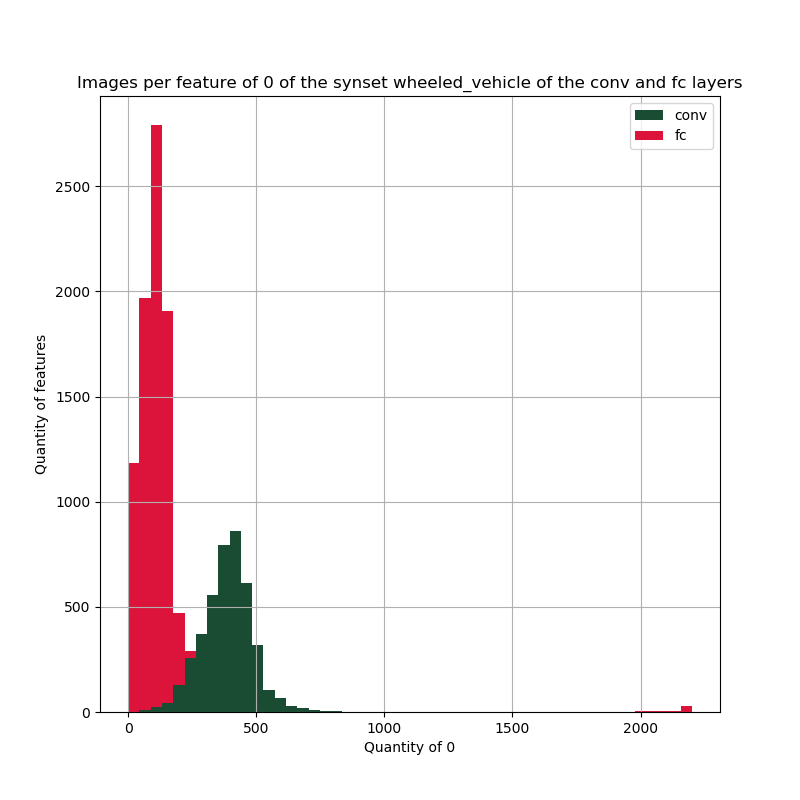
\includegraphics[width=\textwidth]  {Images/plots/25/synsets/Images_per_feature_of_0_category_wheeled_vehicleall_layers.png}
		\caption{Categoría 0}
	\end{subfigure}
	\begin{subfigure}[b]{0.3\textwidth}
		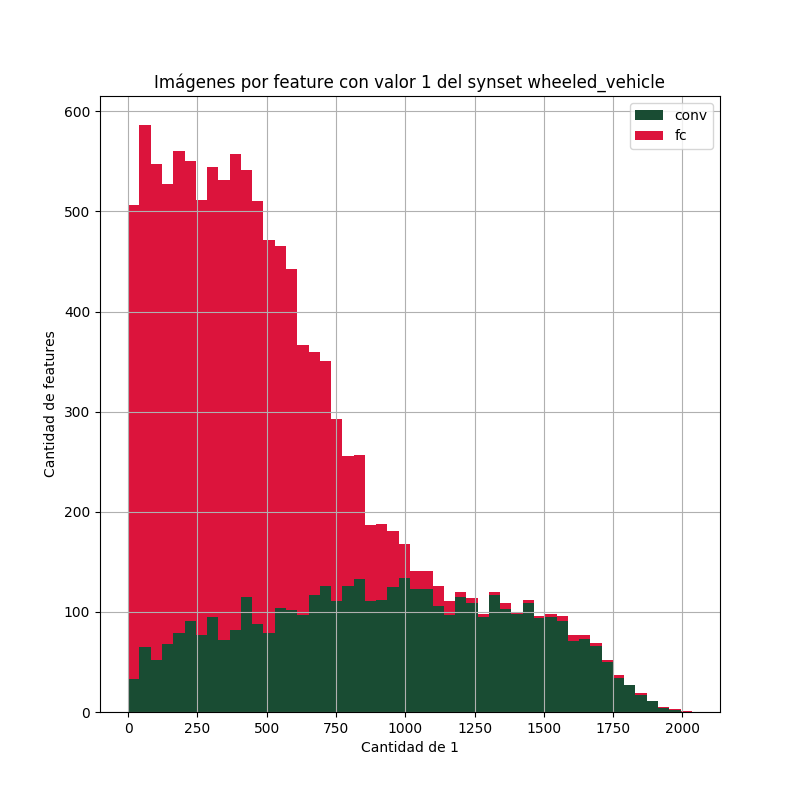
\includegraphics[width=\textwidth]  {Images/plots/25/synsets/Images_per_feature_of_1_category_wheeled_vehicleall_layers.png}
		\caption{Categoría 1}
	\end{subfigure}       
	\caption{Imágenes por categoría del \textit{synset} vehículo \label{fig:imagesperfeaturewheel}}
\end{figure}

La diferencia entre los distintos grupos de gráficas (\textit{synsets} más generales contra más específicos) se debe a que al ser una muestra más pequeña hay una mayor varianza. También se observa una disminución de la proporción de \textit{features} no característica cuanto más concreto es el synset, esto nos da una idea de que la red convolucional se adapta al nivel de generalización que tiene un \textit{synset}, por ejemplo, \textit{perro} tendrá menos \textit{features} no características (en proporción) que \textit{mamífero}. Este hecho concuerda con nuestra hipótesis \ref{h2}, en la que ahondaremos más adelante.

También se observan unos comportamientos simétricos entre las \textit{features} características por presencia y por ausencia en todos los \textit{synsets} y en la gráfica general. Este tipo de simetría es una buena señal, puesto a que la caracterización que hemos dado es abstracta, es decir, la definición de característica por ausencia o por presencia no viene dada por la red convolucional sino por un estudio externo a ésta.  



Otro dato que podemos obtener es la cantidad de \textit{features} de cada una de las categorías por \textit{synset}, como vemos en la figura \ref{fig:totalfeaturespersynset}, simplemente sumando los diferentes valores de las sub-matrices. 


\begin{figure}[ht] 
	\centering
	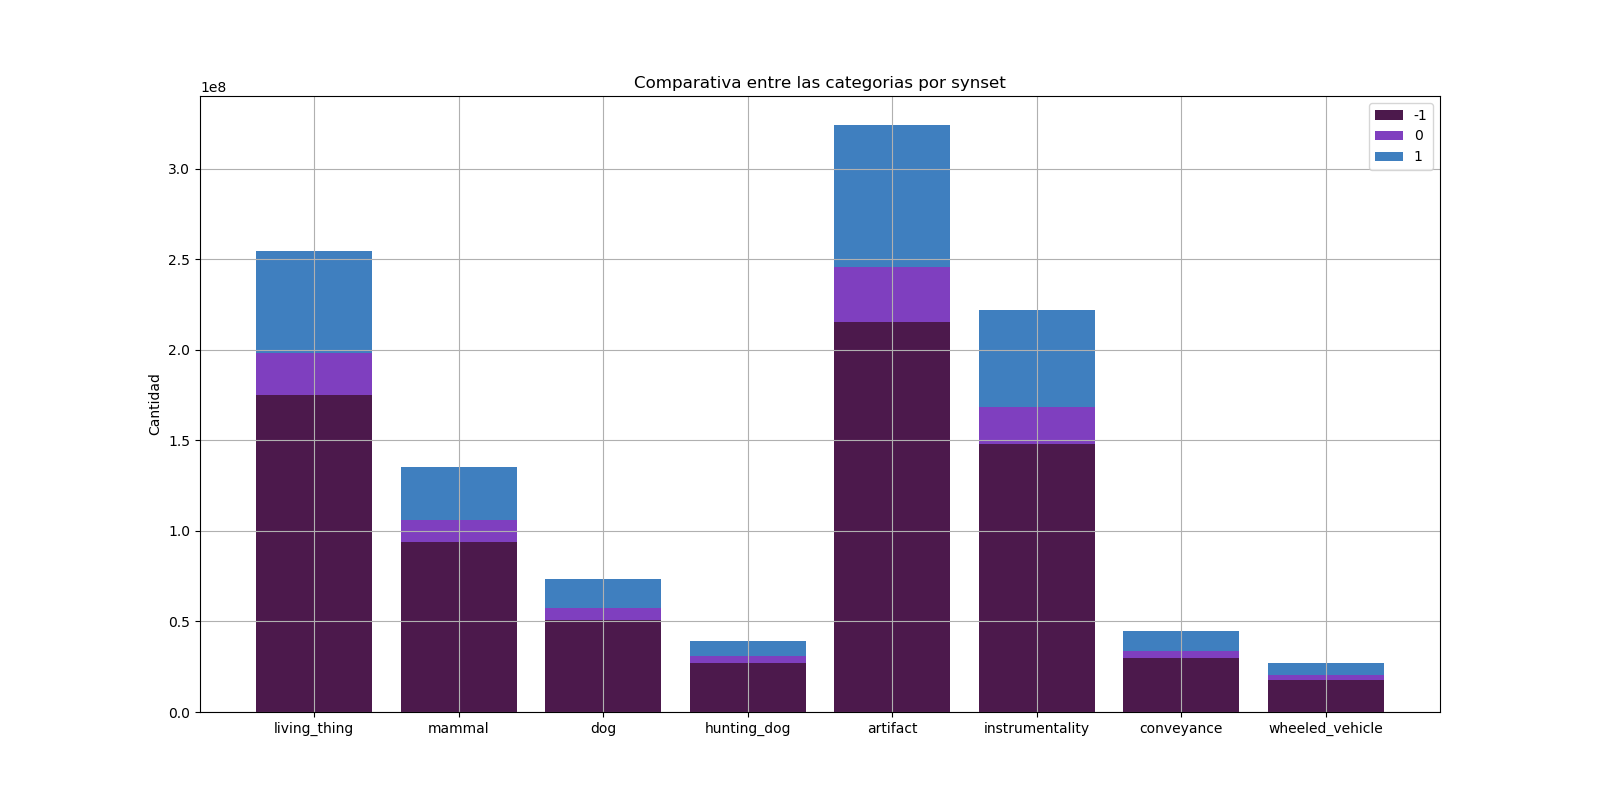
\includegraphics[width=0.9\textwidth] {Images/plots/25/synsetslayer/Comparative_of_synsets_global.png}
	\caption{ Cantidad de features por synset
	\label{fig:totalfeaturespersynset}}
\end{figure}

Además utilizando esta sub-matriz hemos calculado la cantidad de \textit{features} de cada tipo por capa, de la misma forma que calculamos los valores de la gráfica \ref{fig:totalfeaturesperlayer}. En general no se ve mucha diferencia entre las gráficas de cada \textit{synset} y la general( como podemos observar en la figura \ref{fig:featuresperlayervehicle}), esto implica que la cantidad de \textit{features} con los distintos valores por capa es parecida independientemente del synset que tomemos y de lo general que éste sea, cosa que va en contra de nuestra hipótesis \ref{h2}.


\begin{figure}[ht] 
	\centering
	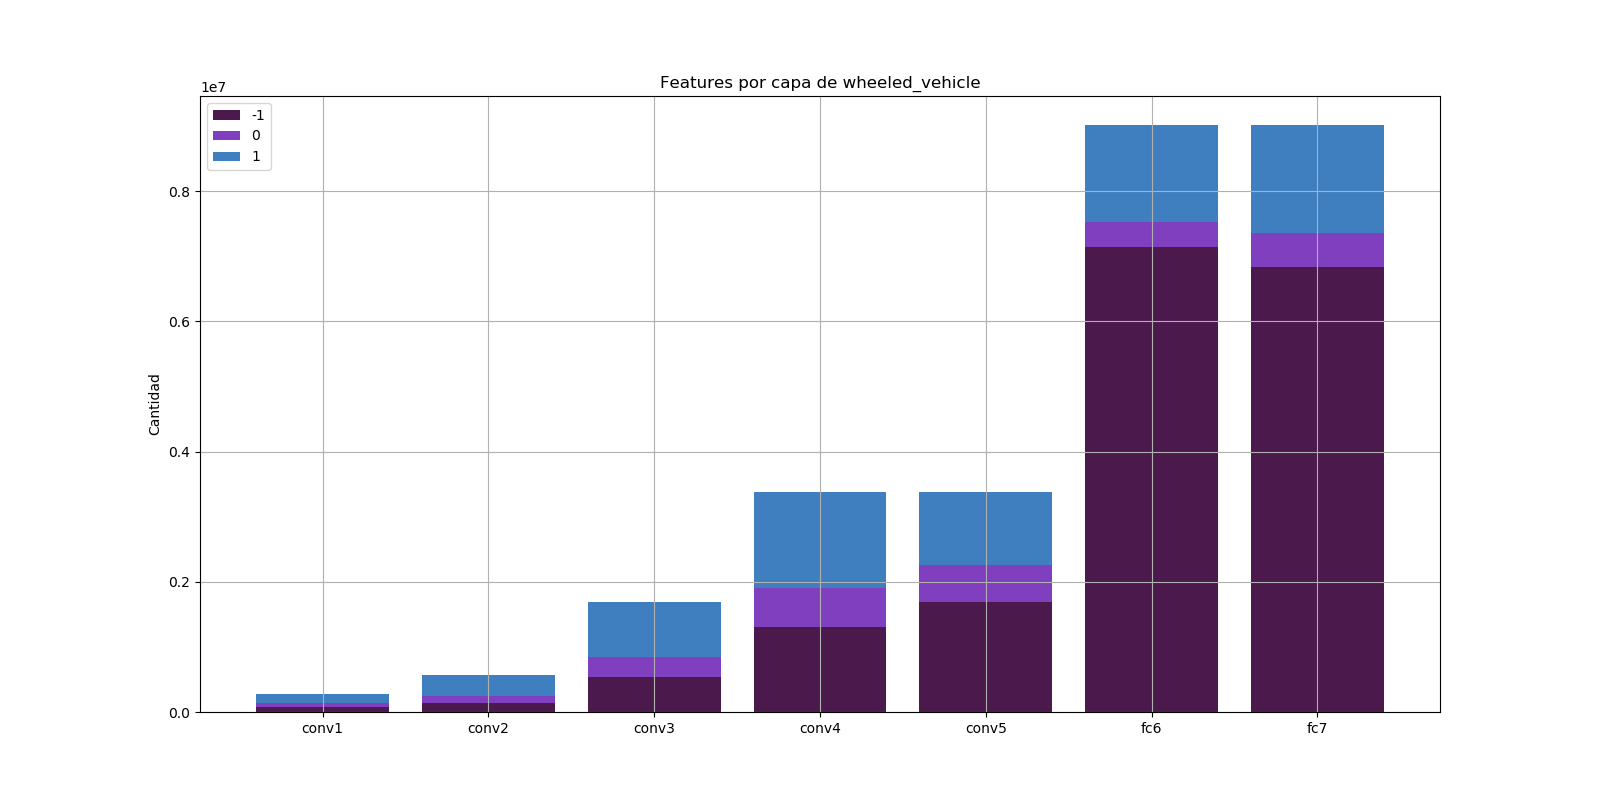
\includegraphics[width=0.9\textwidth] {Images/plots/25/synsetslayer/Comparative_of_synsets_wheeled_vehicle_global.png}
	\caption{ Cantidad de features por capa de vehículo
	\label{fig:featuresperlayervehicle}}
\end{figure}

Mientras que la distribución de las imágenes por \textit{feature} se difuminaba con \textit{synsets} más concretos (figura \ref{fig:imagesperfeaturewheel}), vemos que la proporción de \textit{features} características se conserva, tanto por synset como por capa. Esto nos confirma que la difuminación que veíamos sea debida a una menor cantidad de muestras a la hora de calcular la gráfica y no a una distinción por \textit{synset}. 

\textbf{Representante:}

Con la sub-matriz hemos logrado una visión general del comportamiento de los \textit{synsets} dentro del \textit{embedding}, pero hay información que estamos perdiendo. Sería interesante saber si a nivel de \textit{feature} diferentes \textit{synsets} se comportan distinto, o de la misma forma, como parecían indicar los descubrimientos para sub-matrices. Por ejemplo que se concentrasen todos los 1 en un mismo conjunto de \textit{features} para el mismo synset.

Para solventar este problema decidimos tomar un vector muestra para cada uno de los \textit{synsets} de tamaño $1x12,416$ donde cada componente se toma como la categoría más frecuente para esa \textit{feature} concreta, como muestra la figura \ref{fig:representante}. 
 
\begin{figure}[ht]
\begin{center}
%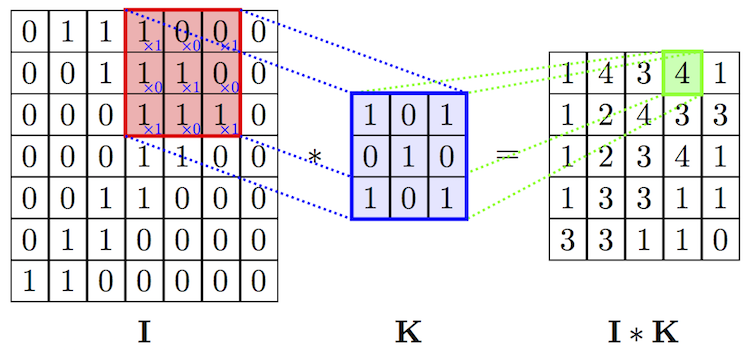
\includegraphics[width = 0.5\textwidth]{Images/convolve.png} 
\begin{tikzpicture}

	\matrix (mtr) [matrix of nodes,column sep=-\pgflinewidth, row sep=-\pgflinewidth,  nodes={draw,
      minimum height=0.5cm,
      anchor=center,
      text width=0.5cm,
      align=center,
      inner sep=0pt
    }]
	{
		|[fill=blue!30]| 1 & |[fill=blue!30]| -1 & |[fill=blue!30]| -1 & |[fill=blue!30]| 1 & |[fill=blue!30]| 0 & |[fill=blue!30]| 0 & |[fill=blue!30]| -1\\
		0 & 0 & -1 & -1 & -1 & 0 & 0\\
		0 & 0 & 0 & 1 & -1 & -1 & 0\\
		|[fill=green!30]| 0 & |[fill=green!30]| 1 & |[fill=green!30]| -1 & |[fill=green!30]| 1 & |[fill=green!30]| 1 & |[fill=green!30]| 0 & |[fill=green!30]| 0\\
		|[fill=blue!30]| 1 & |[fill=blue!30]| 1 & |[fill=blue!30]| -1 & |[fill=blue!30]| 0 & |[fill=blue!30]| -1 & |[fill=blue!30]| 0 & |[fill=blue!30]| 0\\
		0 & 0 & -1 & 1 & 0 & 0 & 0\\
		0 & -1 & 1 & 0 & 0 & 0 & 1\\
		|[fill=blue!30]| 1 & |[fill=blue!30]| 1 & |[fill=blue!30]| 1 & |[fill=blue!30]| -1 & |[fill=blue!30]| -1 & |[fill=blue!30]| 0 & |[fill=blue!30]| 0\\
		-1 & -1 & 0 & 0 & 0 & 0 & 0\\
	};
    \node [below= of mtr-7-4.south] (lm) {embedding};


	\matrix (K) [right=5em of mtr,matrix of nodes,row sep=-\pgflinewidth, nodes={draw, fill=blue!30}]
	{
		1 & 1 & -1 & 1 & -1 & 0 & 0\\
	};
	
    \node [below= of K-1-4.south] (lk) {representante};

    \draw[very thick, blue] (K-1-1.north west) rectangle (K-1-7.south east);
	
	\draw[densely dotted, blue, thick] (mtr-1-1.north west) -- (K-1-1.north west);
	\draw[densely dotted, blue, thick] (mtr-1-1.south west) -- (K-1-1.south west);
	\draw[densely dotted, blue, thick] (mtr-1-7.north east) -- (K-1-7.north east);
	\draw[densely dotted, blue, thick] (mtr-1-7.south east) -- (K-1-7.south east);
	
	\draw[densely dotted, blue, thick] (mtr-5-1.north west) -- (K-1-1.north west);
	\draw[densely dotted, blue, thick] (mtr-5-1.south west) -- (K-1-1.south west);
	\draw[densely dotted, blue, thick] (mtr-5-7.north east) -- (K-1-7.north east);
	\draw[densely dotted, blue, thick] (mtr-5-7.south east) -- (K-1-7.south east);
	
    \draw[densely dotted, blue, thick] (mtr-8-1.north west) -- (K-1-1.north west);
	\draw[densely dotted, blue, thick] (mtr-8-1.south west) -- (K-1-1.south west);
	\draw[densely dotted, blue, thick] (mtr-8-7.north east) -- (K-1-7.north east);
	\draw[densely dotted, blue, thick] (mtr-8-7.south east) -- (K-1-7.south east);
%	\draw[very thick, blue] (K-1-1.north west) rectangle (K-3-3.south east);

\end{tikzpicture}
\end{center}
\caption{Ejemplo de un representante de \textit{synset}.
\label{fig:representante}}
\end{figure}

De esta obtenemos una información más concreta respecto a cada \textit{feature}, además podemos comparar los distintos \textit{synsets} de una forma más efectiva. Por ejemplo, si una \textit{feature} suele ser característica para mamíferos, quedará marcada en el representante, mientras que si tomáramos los valores de la proporción de las características respecto a la sub-matriz correspondiente al \textit{synset} esta información se perdería, ya que la proporción de \textit{features} no características es muy superior a la del resto de opciones.

Al calcular las gráficas anteriores, pero del representante, esta vez si que obtenemos diferencias. 

Primero de todo observamos que en la gráfica \ref{fig:comparativaCategoriasporSynset}, cuanto más concreto es el \textit{synset} mayor proporción de features características por presencia tenemos, además que las \textit{features} no características desaparecen prácticamente por completo. Esto implica que las \textit{features} no características no sólo están en minoría para la mayoría de imágenes y \textit{features},sino que además no se concentran en conjuntos concretos de \textit{features}.   
\begin{figure}[ht] 
	\centering
	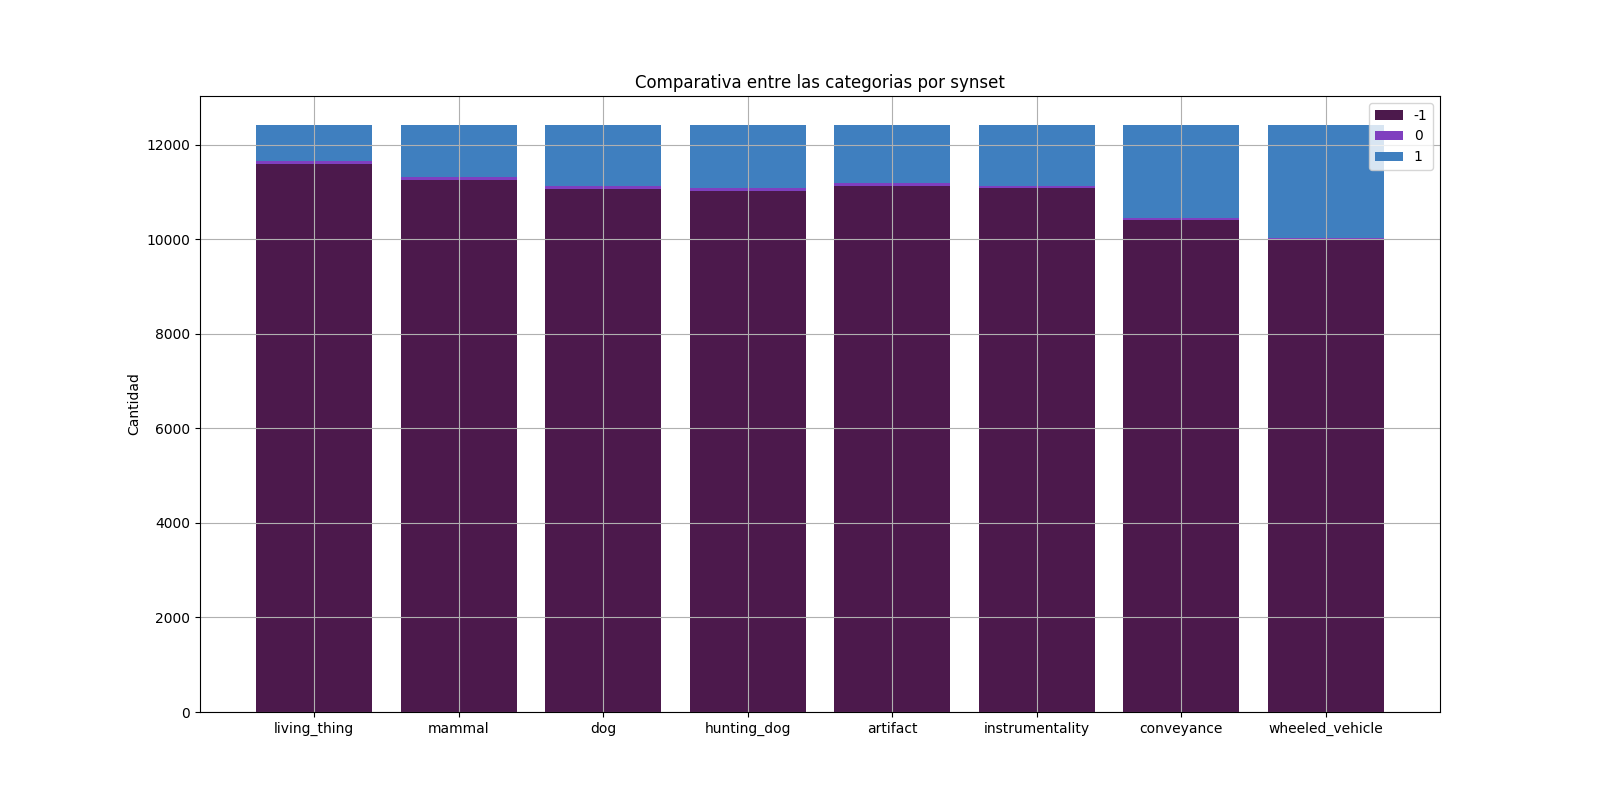
\includegraphics[width=0.9\textwidth] {Images/plots/25/synsetslayer/Comparative_of_synsets.png}
	\caption{ Cantidad de features de los representantes
	\label{fig:comparativaCategoriasporSynset}}
\end{figure}

Si además comparamos la gráfica \ref{fig:comparativaCategoriasporSynset} con la de \ref{fig:totalfeaturespersynset} vemos que las features características aparecen en mayor proporción. Si no estuvieran concentradas, las \textit{features} tomarían todas el valor -1, puesto a que es el más común en el embedding. 
\begin{figure}[ht] 
	\centering
	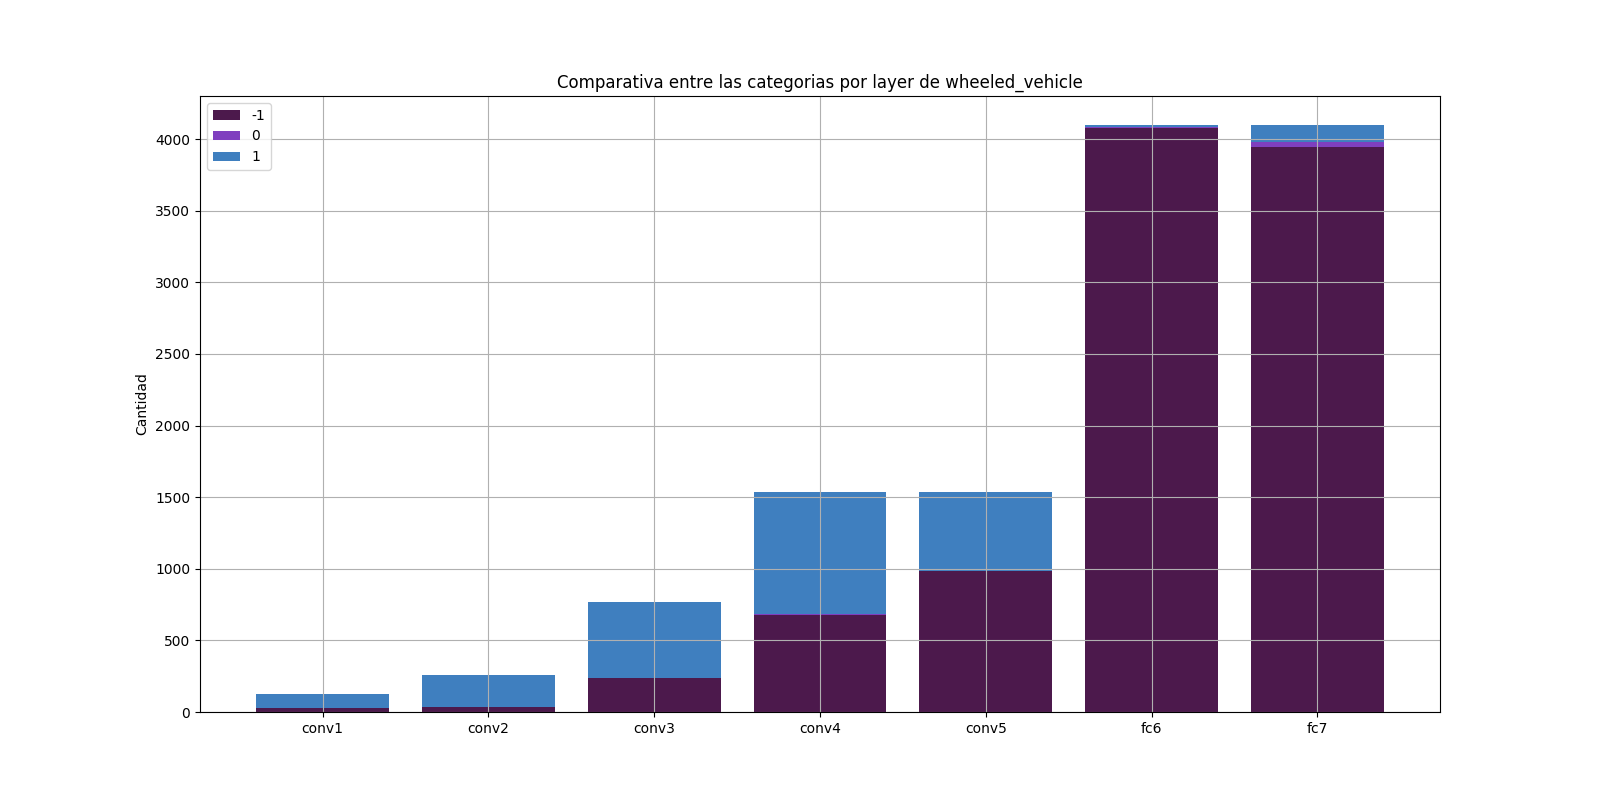
\includegraphics[width=0.9\textwidth] {Images/plots/25/synsetslayer/Comparative_of_synsets_wheeled_vehicle.png}
	\caption{ Cantidad de features de los representantes
	\label{fig:comparativaVehiculo}}
\end{figure}

Respecto a las proporciones por capa, para todos los synsets han salido resultados parecidos, siendo el más visible el correspondiente a Vehículo, como  vemos en la \ref{fig:comparativaVehiculo}. En este caso también vemos una desaparición de las \textit{features} no representativas en todas las capas. 
Además la proporción de \textit{features} características aumenta en las capas convolucionales, mientras que disminuye en las \textit{fully-connected}. Lo que implica una dispersión de los valores característicos con respecto a los que no lo son. 

Para comparar los \textit{synsets} a un nivel todavía más concreto hemos generado diferentes matrices de cambio a partir de los representantes, éstas están definidas como vemos en la figura \ref{fig:matrizss1ss2}. 
 \begin{figure}[ht] 
	\centering
	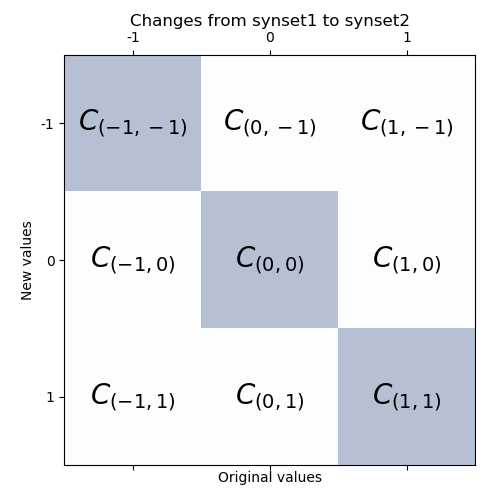
\includegraphics[width=0.4\textwidth] {Images/plots/25/matrices/Changesfromsynset1tosynset2.png}
	\caption{ Matriz de cambios
	\label{fig:matrizss1ss2}}
\end{figure}

Donde $C_{(i,j)}$ es la cantidad de valores que en el primer \textit{synset} valían $i$ y en el segundo valen $j$, comparando elemento a elemento. La suma total de todas las $C_{(i,j)}$ es 12,416, es decir, la cantidad total de \textit{features} de un representante. Además, si sumamos todas las $C_{(i,j)}$ de una columna concreta obtenemos el total de \textit{features} con valor $i$ del primer \textit{synset}, y de forma simétrica, si sumamos las filas obtenemos el total de \textit{features} con valor $j$ del segundo \textit{synset}.


En la diagonal contienen la cantidad de valores que se conservan, es decir, que para el primer \textit{synset} y el segundo tienen el mismo valor. En el resto de posiciones contiene la cantidad de \textit{features} que en el primer \textit{synset} tenían un valor y en el segundo pasa a tener otro.

En nuestro primer ejemplo de matrices de cambio (figura \ref{fig:matrixliving}) podemos observar que, tanto la columna como la fila correspondiente al cero (las \textit{features} no características) tiene unos valores muy bajos con respecto al resto. Esto se repite en todas las matrices para todos los \textit{synsets}, puesto a que el total de \textit{features} con este valor es muy bajo. Respecto al resto de valores, los explicaré por columnas para facilitar la comprensión. 

En la columna de las \textit{features} características por ausencia se acumulan la mayoría de los valores, como era de esperar. En la figura \ref{fig:matrixlivinginstrum}, vemos una respetable cantidad de \textit{features} que eran representativas por ausencia para seres vivos pasan a ser representativas por presencia en \textit{instrumentos}, además, este fenómeno se acentua en \textit{synsets} más concretos, como vemos en la figura \ref{fig:matrixlivingwheel}. Un ejemplo de este comportamiento podrían ser \textit{features} que detectaran ruedas, a la hora de clasificar, sería representativo para seres vivos que no tuvieran ruedas, mientras que el \textit{synset} de los instrumentos, contiene los vehículos, para los que esta \textit{feature} sería característica por presencia.   
Para Perro de caza, sin embargo, la cantidad de \textit{features} de valor -1 que pasan a valer 1, es significativamente menor. Las que hay podrían ser \textit{features} bastante concretas, que se asociaran a perros de caza, pero no al conjunto general de seres vivos, como por ejemplo ser cierta raza de perro. 

Finalmente en la columna de las \textit{features} características por presencia, vemos en la figura en al que se conservan más es \ref{fig:matrixlivinghunting}, mientras que en el resto casi todas pasan a ser características por ausencia. De forma simétrica al comportamiento de la columna de las \textit{features} características por ausencia, pero a menor escala. 
 \begin{figure}[ht] 
	\centering
	\begin{subfigure}[b]{0.3\textwidth}
		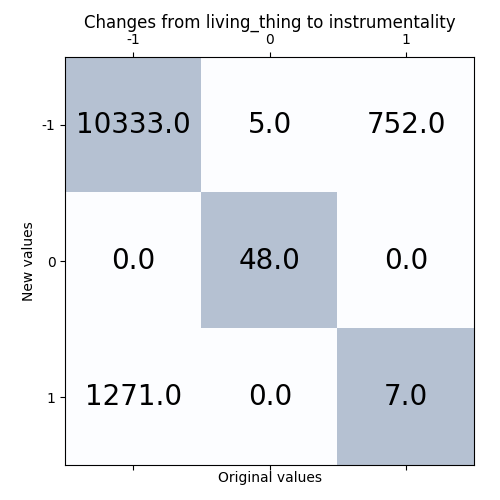
\includegraphics[width=\textwidth] {Images/plots/25/matrices/matrixlivinginstrum.png}
		\caption{Ser Vivo a Instrumento \label{fig:matrixlivinginstrum}}
	\end{subfigure}
	\begin{subfigure}[b]{0.3\textwidth}
		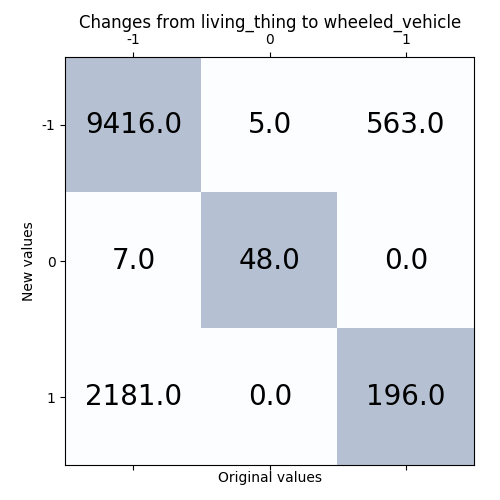
\includegraphics[width=\textwidth]  {Images/plots/25/matrices/matrixLivingWheel.png}
		\caption{Ser Vivo a Vehículo \label{fig:matrixlivingwheel}}
	\end{subfigure}
	\begin{subfigure}[b]{0.3\textwidth}
		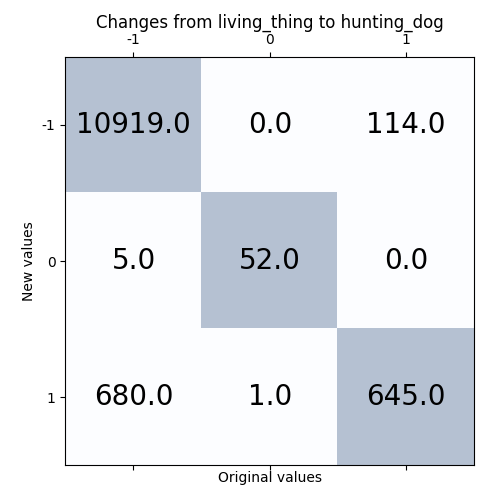
\includegraphics[width=\textwidth]  {Images/plots/25/matrices/matrixLivingHunting.png}
		\caption{Ser Vivo a Perro de Caza \label{fig:matrixlivinghunting}}
	\end{subfigure}       
	\caption{Matrices de cambio de Ser Vivo \label{fig:matrixliving}}
\end{figure}

El siguiente ejemplo (\ref{fig:matrixconcret}) es para ver el comportamiento en \textit{synsets} más concretos. Podemos ver claramente que la red está captando la similitud entre Perro y Perro de caza, puesto a que casi todas las \textit{features} se mantienen en la diagonal. Se comporta de forma parecida con Transporte y Vehículo. Mientras que entre Perro de Caza y Vehículo la mayoría de las \textit{features} pasan de características a no características y viceversa. Nótese la similitud de la figura \ref{fig:MatrixWheelHunt} y la figura \ref{fig:matrixlivinginstrum}, aun siendo en el primer caso los synsets más concretos y en el segundo los más generales, el comportamiento es parecido.

\begin{figure}[ht] 
	\centering
	\begin{subfigure}[b]{0.3\textwidth}
		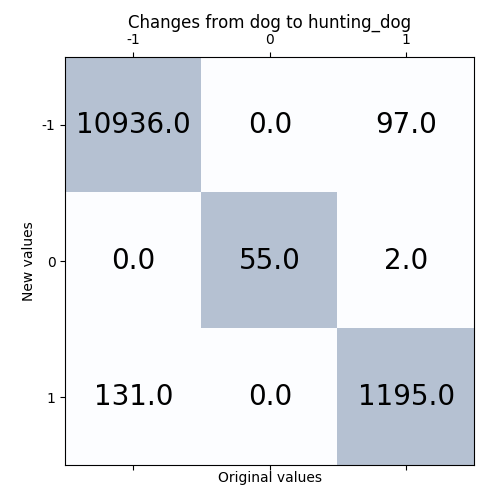
\includegraphics[width=\textwidth] {Images/plots/25/matrices/MatrixDogHunting.png}
		\caption{Perro a Perro de caza \label{fig:MatrixDogHunting}}
	\end{subfigure}
	\begin{subfigure}[b]{0.3\textwidth}
		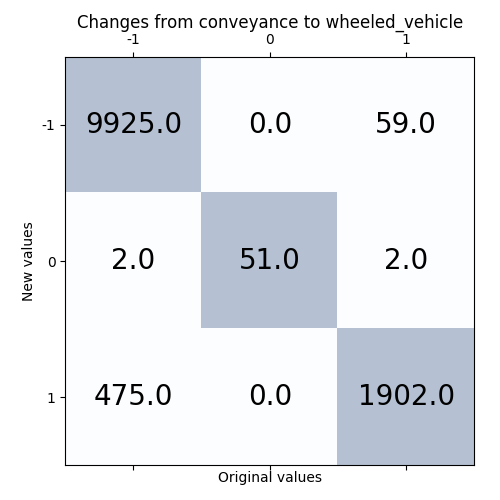
\includegraphics[width=\textwidth]  {Images/plots/25/matrices/matrixConveyanceWheel.png}
		\caption{Transporte a Vehículo \label{fig:matrixConveyanceWheel}}
	\end{subfigure}
	\begin{subfigure}[b]{0.3\textwidth}
		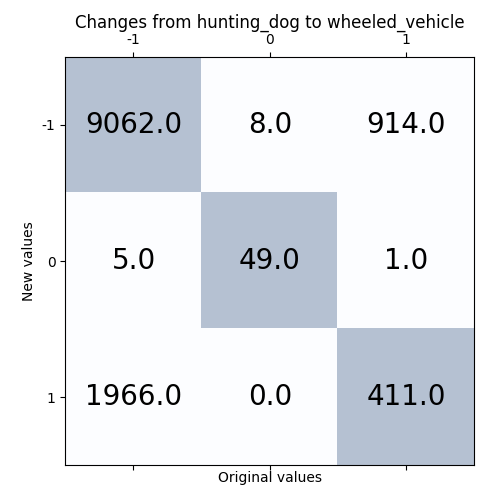
\includegraphics[width=\textwidth]  {Images/plots/25/matrices/matrixhuntingwheel.png}
		\caption{Perro de caza a Vehículo\label{fig:MatrixWheelHunt}}
	\end{subfigure}       
	\caption{Matrices de cambio\label{fig:matrixconcret}}
\end{figure}


\subsection{Del full network embedding a wordnet}

%Explicación de la distancia definida entre los synsets, demostración de que es distancia, los grafos con las distancias. 

Partiendo de los resultados del apartado \ref{sec:synsets} hemos generado una distancia que representa lo diferentes que son cada uno de los \textit{synsets} que aparecen en \textit{imagenet} para la red convolucional entrenada. En este apartado explicaremos como se ha obtenido y como se relaciona con lo estudiado en el apartado anterior. 

Para empezar, definimos los siguientes conjuntos.
\begin{definition}
Llamaremos $\mathfrak{C}$ al conjunto de \textit{synsets} correspondientes a cada una de las  1,000 clases posibles en las que clasifica nuestra red convolucional.  

Llamaremos $\mathfrak{I}$ al conjunto de todos los \textit{synsets} que pertenecen a $\mathfrak{C}$ junto con todos los \textit{synsets} de \textit{wordnet} que tienen algún hipónimo en $\mathfrak{C}$. 

Al conjunto de \textit{synsets} de \textit{wordnet} lo denotaremos $\mathfrak{W}$. 
\end{definition}

Por construcción tenemos: 

\begin{equ}[H]
\begin{equation*}
\mathfrak{C} \subset \mathfrak{I} \subset \mathfrak{W}
\end{equation*}
\end{equ}

Nuestro objetivo es construir una métrica para $\mathfrak{I}$ que dependa de la red convolucional entrenada. Para de esta forma poder medir lo diferentes que son dos \textit{synsets} en términos de la red. 

Para ello recordamos la definición de métrica:
\begin{definition}
Sea $X$ un conjunto, una \textbf{métrica} o distancia es una función:
$$
d:X\times X \rightarrow [0,\infty)\subset \mathbb{R}
$$

Donde dados $x,y,z\in X$ se cumple:
\begin{enumerate}
\item $d(x,y) \geq 0$
\item $d(x,y)=0 \iff x=y $ \label{indiscernibles}
\item $d(x,y) = d(y,x)$
\item $d(x,z) \geq d(x,y) + d(y,z)$
\end{enumerate}
\end{definition}

La forma natural de conectar diferentes \textit{synsets} sería a partir de un árbol utilizando las conexiones de hiponimia e hiperonimia, similar la de la figura \ref{fig:hiponimos} y utilizar la distancia discreta. Sin embargo, una distancia que utilizase solamente esta información no dependería de la red. 

Para solventar este problema utilizamos la información obtenida en la sección \ref{sec:synsets}, donde vimos que se podía definir matrices de cambio a partir de los representantes de cada \textit{synset}. Estas matrices nos pueden dar una idea de lo parecidos que son dos \textit{synsets} en términos de la red. 

Otro problema que nos encontramos es que, de la forma en la que hemos definido $\mathfrak{I}$ se puede dar el caso de que dos \textit{synsets} diferentes tengan las mismas \textit{features} (y en consecuencia la misma matriz). Por ejemplo, si tomamos un \textit{synset} que sólo contenga un hipónimo en $\mathfrak{C}$ y lo comparamos con éste, los dos tendrían exactamente el mismo vector representante. Esto hace que no podamos utilizar la definición de métrica estándar, puesto a que fallaría la propiedad \ref{indiscernibles}, así que utilizaremos una \textbf{pseudométrica}.

\begin{definition}
Sea $X$ un conjunto, una \textbf{pseudo-métrica} es una función:
$$
d:X\times X \rightarrow [0,\infty)\subset \mathbb{R}
$$

Donde dados $x,y,z\in X$ se cumple:
\begin{enumerate}
\item $d(x,y) \geq 0$
\item $d(x,x)=0$ 
\item $d(x,y) = d(y,x)$
\item $d(x,z) \geq d(x,y) + d(y,z)$
\end{enumerate}
\end{definition}

 Como nuestro objetivo es medir lo diferentes que son los \textit{synsets} para la red, una pseudo-métrica es suficiente. La definiremos 
utilizando la notación introducida en la figura \ref{fig:matrizss1ss2}: 

\begin{equ}[H]
\begin{equation*}
d(s_1,s_2) = 1 - \frac{C_{(1,1)}(s_1,s_2)}{C_{(1,-1)}(s_1,s_2) + C_{(1,0)}(s_1,s_2) + C_{(1,1)}(s_1,s_2) + C_{(1,1)}(s_1,s_2) + C_{(0,1)}(s_1,s_2) + C_{(-1,1)}(s_1,s_2)}
\end{equation*}
\caption{Distancia entre el \textit{synset} $s_1$ y el $s_2$ \label{eq:distance}}
\end{equ}
Donde $s_1, s_2 \in \mathfrak{I}$. Es trivial comprobar que esta función cumple las propiedades necesarias para ser pseudo-métrica. Puesto a que se basa en una proporción, los valores de la pseudo-métrica estarán entre cero y uno. 

Esta distancia corresponde a la proporción de \textit{features} características por presencia que se conservan entre $s_1$ y $s_2$ respecto a la suma de \textit{features} características por presencia de los dos \textit{synsets}.
De esta manera podemos medir la similitud de dos \textit{synsets} respecto al \textit{embedding} y por tanto, respecto a la red convolucional entrenada.

Si la utilizamos para comparar los ejemplos de las figuras \ref{fig:matrixliving} y \ref{fig:matrixconcret} tenemos las siguientes distancias: 
\begin{align*}
d(\text{Ser vivo, Instrumento}) &= 0.9965 & d(\text{Ser vivo, Vehículo}) &= 0.9333 \\ 
d(\text{Ser vivo, Perro de caza}) &= 0.5520 & d(\text{Perro, Perro de caza}) &= 0.1614 \\
d(\text{Transporte, Vehículo}) &= 0.2201 & d(\text{Perro de caza, Vehículo}) &=0.8751 & 
\end{align*}
	
Donde vemos claramente que capta bien la similitud entre los distintos \textit{synsets}, siendo los más diferentes entre si Ser vivo e Instrumento y los más similares perro y perro de caza. 

Para terminar de visualizar las distancias hemos generado el árbol de hipónimos de diferentes \textit{synsets} utilizando la psedudo-métrica definida como distancia entre los nodos. Para ello hemos hecho un BFS en el grafo de \textit{wordnet} tomando como aristas la relación de hiponimia y como nodo padre el \textit{synset} del que queríamos generar el árbol.Se podrían obtener también las distancias entre el resto de nodos y generar un grafo completo, pero esto dificultaría la visualización, y en consecuencia, la obtención de conclusiones. 

Un ejemplo de ello sería la figura \ref{fig:grafoperro}, donde vemos que la distancia entre Perro con Perro de caza, y Perro con Perro de trabajo son inferiores que las de razas concretas de perro con sus respectivos hiperónimos. Lo que significa que, dentro del conjunto de perros, para la red se parecen más \textit{synsets} más generales que razas concretas.


Para tener una idea de las relaciones entre razas concretas hemos calculado todas las distancias entre los diferentes \textit{synsets} del conjunto de hipónimos de Perro de caza. Un ejemplo de ello serían las razas de la figura \ref{fig:dogexample}, donde vemos tres razas de perro claramente diferenciadas. 

\begin{figure}[H] 
	\centering
	\begin{subfigure}[b]{0.3\textwidth}
		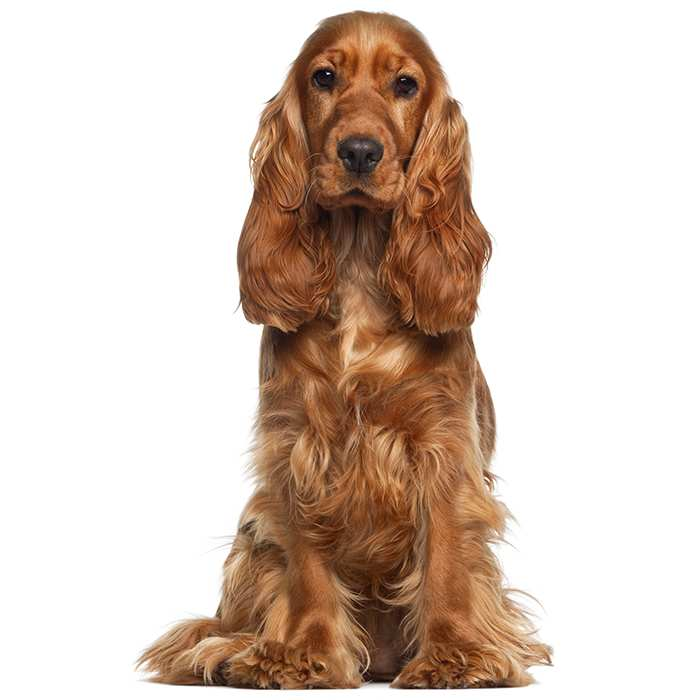
\includegraphics[height=4cm] {Images/examples/spaniel.jpg}
		\caption{Spaniel \label{fig:spaniel}}
	\end{subfigure}
	\begin{subfigure}[b]{0.3\textwidth}
		\centering
		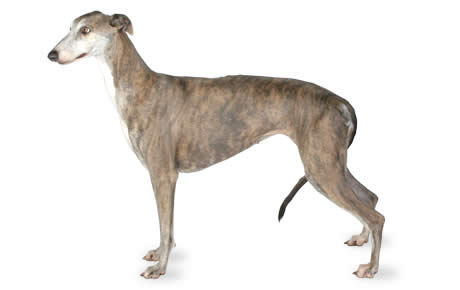
\includegraphics[height=4cm]  {Images/examples/greyhound.jpg}
		\caption{Greyhound \label{fig:greyhound}}
	\end{subfigure}
	\begin{subfigure}[b]{0.3\textwidth}
		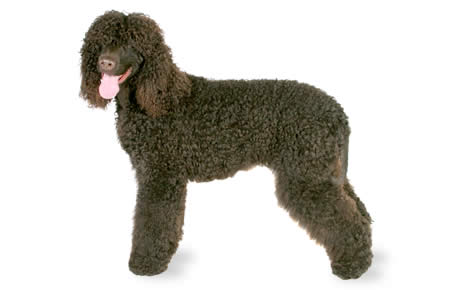
\includegraphics[height=4cm]{Images/examples/waterspaniel.jpg}
		\caption{Water Spaniel\label{fig:waterspaniel}}
	\end{subfigure}       
	\caption{Ejemplos de razas\label{fig:dogexample}}
\end{figure}

Sus respectivas distancias son: 

\begin{table}[H]
\centering
\caption{Distancias entre las razas del ejemplo}
\label{tabledogs}
\begin{tabular}{l|l|l|l}
              & Spaniel & Grayhound & Water Spaniel               \\ \hline
Spaniel       & 0       & 0.7371    & \multicolumn{1}{l|}{0.6442} \\ \hline
Grayhound     & 0.7371  & 0         & \multicolumn{1}{l|}{0.8330} \\ \hline
Water Spaniel & 0.6442  & 0.8330    & \multicolumn{1}{l|}{0}      \\ \cline{2-4} 
\end{tabular}
\end{table}

En la tabla \ref{tabledogs} podemos ver que el Spaniel se parece más al Water-spaniel que al Grayhound, cosa que es coerente con la imagen \ref{fig:dogexample}. 
 

 \begin{figure}[H] 
	\centering
	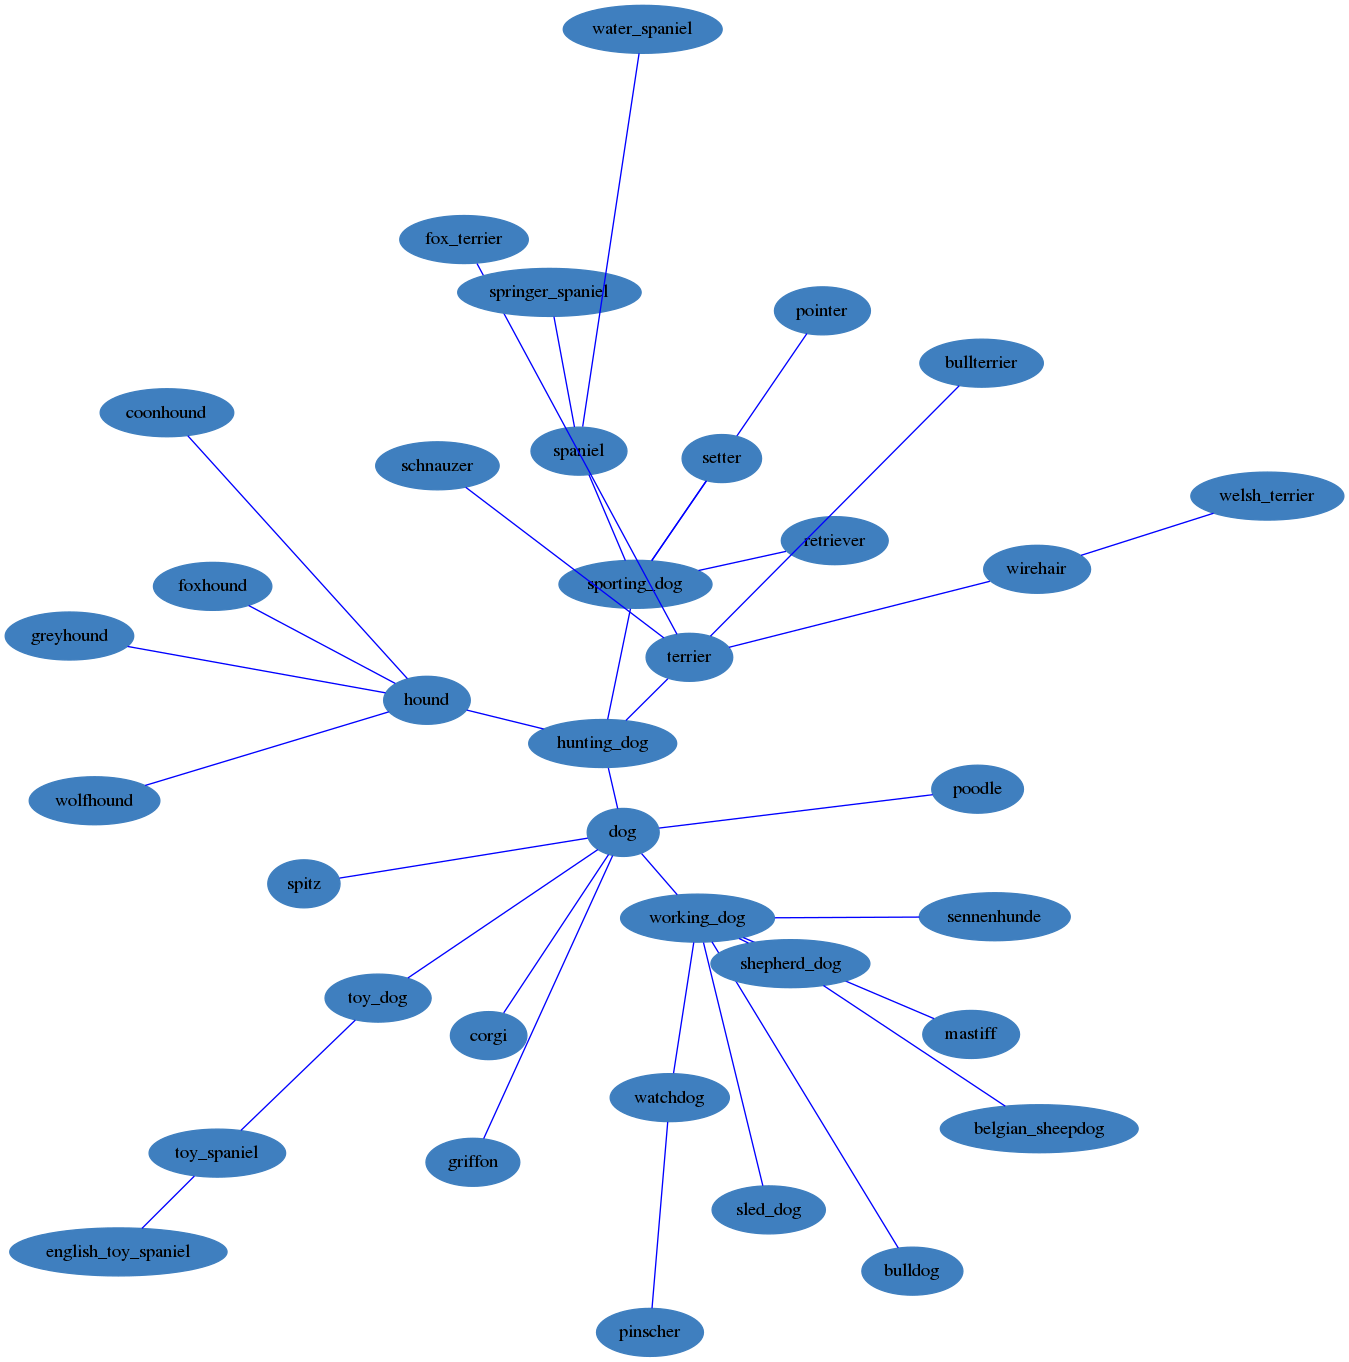
\includegraphics[width=0.9\textwidth] {Images/forest/dog.png}
	\caption{ Árbol del \textit{synset} perro
	\label{fig:grafoperro}}
\end{figure}

\newpage

\section{Conclusiones}

En esta sección explicaremos las conclusiones obtenidas a partir de las secciones anteriores. Además revisaremos las hipótesis planteadas en \ref{sec:enfoque}. Los puntos base de la concusión son los siguientes: 

\begin{itemize}
\item Las capas \textit{fully-connected} tienen una distribución diferente de las convolucionales, tanto a nivel general como por \textit{synset}. Lo que implica que aun después de la estandarización hecha a las capas convolucionales, éstas mantienen sus diferencias respecto a las \textit{fully-connected}. Además en todas las distribuciones se ve una cierta simetría entre las gráficas de la categoría de las \textit{features} representativas por ausencia y las representativas por presencia. Por estos motivos aceptamos la hipótesis \ref{h1}.

\item Las \textit{features} no características no solo son minoría, sino que además no están concentradas para ninguna \textit{feature} concreta. De esta forma vemos que todas las \textit{features} contienen información que caracteriza el espacio de representación. 

\item La proporción de las \textit{features} características por ausencia, presencia o no características se mantiene tanto por capa como por synset. Sin embargo, en el estudio utilizando representantes hemos visto que estas se distribuyen en grupos, es decir, aunque en la proporción global las \textit{features} características por ausencia siempre son mayoría, para ciertas \textit{features} hay una mayoría de \textit{features} características por presencia, y por tanto las proporciones son significativamente diferentes a nivel de representante, donde se observan los siguientes fenómenos: 

\begin{itemize}
\item Las \textit{features} representativas por presencia se concentran en las capas convolucionales, sobretodo en la cuarta y la quinta. Mientras que en las \textit{fully-connected} se concentran las representativas por ausencia. 
\item Cuanto más concreto es el \textit{synset} mayor proporción de \textit{features} representativas contiene. 
\end{itemize}

Puesto a que la proporción a nivel global era similar tanto en las capas como en los \textit{synsets} esto significa que, a diferencia de lo que pensábamos en un primer lugar,en las capas convolucionales cuanto más concreto es el \textit{synset} o más profunda es la capa más se agrupan las \textit{features} características por presencia en \textit{features} concretas. Esto nos hace revocar las hipótesis \ref{h2} y \ref{h3}.

\item El \textit{embedding} detecta similitud a nivel de \textit{synset}. Si comparamos representantes de diferentes \textit{synsets} observamos que entre \textit{synsets} cercanos a nivel de hiponimia e hipernimia coinciden muchas más \textit{features} que en \textit{synsets} lejanos. Por tanto aceptamos la hipótesis \ref{h4}
\item Utilizando la pseudo-métrica definida podemos medir esta distancia y representarla gráficamente. De esta forma obtenemos información sobre como está decidiendo que clase corresponde a que imagen. Por ejemplo, entre mamífero y mamífero acuático(figura \ref{fig:wordnetexample}) se veía una gran distancia. Al comparar ambos conjuntos de imágenes se puede ver que mientras los mamíferos acuáticos tienen fondo azul por el mar, los mamíferos suelen contener colores más marrones o verdes. De esta forma podemos ver que algo que está teniendo en cuenta para clasificar es si están en el mar o no.
\end{itemize}

\begin{figure}[H] 
	\centering
	\begin{subfigure}[b]{0.43\textwidth}
		
		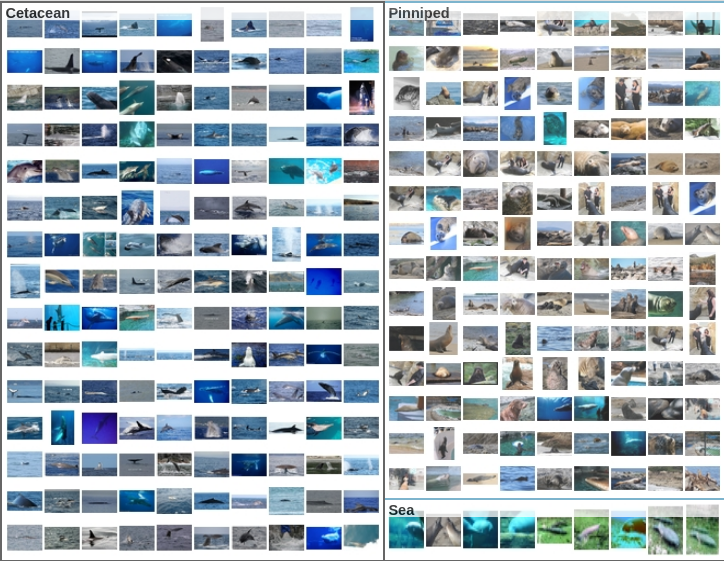
\includegraphics[width=\textwidth] {Images/imagenet/aquatic_mamal.png}
		\caption{Mamífero Acuático \label{fig:aquaticmammal}}
	\end{subfigure}
	\begin{subfigure}[b]{0.43\textwidth}
		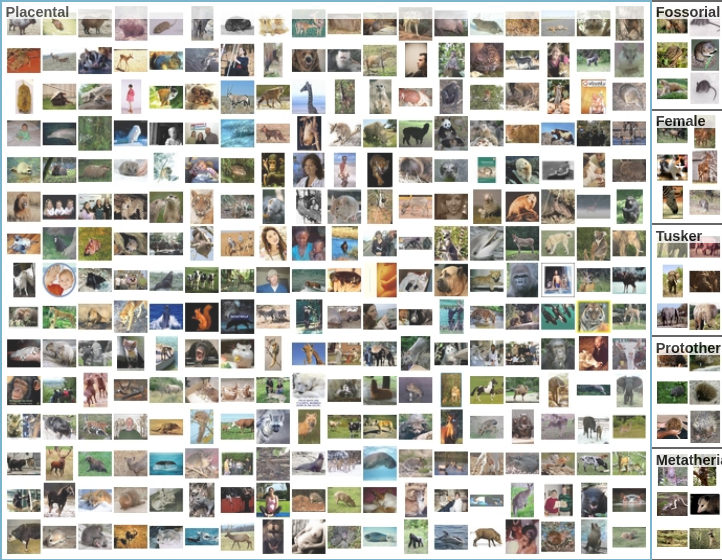
\includegraphics[width=\textwidth]{Images/imagenet/mammal.png}
		\caption{Mamífero\label{fig:mammal}}
	\end{subfigure}       
	\caption{Ejemplos de synsets\label{fig:wordnetexample}}
\end{figure}


%La idea principal de tfg es buscar relaciones entre los synsets de wordnet y el full network embedding. 
%Hipótesis iniciales: 
%- cuanto más concreto sea el synset más 1 debería tener.
%- Cuanto más profundo sea el layer más 1.


%\section{Estructura del TFG: }
%
%\begin{itemize}
%\item \textbf{Introducción (5 pags): }
%\begin{itemize}
%\item FNN (Explicar neural networks, me puedo inspirar en \url{https://upc-mai-dl.github.io/mlp-convnets-theory/})
%\item CNN 
%\item EMbeddings  (Transfer Learning)
%\end{itemize}
%\item \textbf{Related Work (10 pags):}
%\begin{itemize}
%\item FNE 
%\item Wordnet 
%\item imagenet 
%\end{itemize}
%\item \textbf{Approach }
%\begin{itemize}
%\item Hipotesis iniciales 
%\item statistics 
%\item insights 
%\end{itemize}
%\item \textbf{Analysis}
%\begin{itemize}
%\item De wordnet a fne: Dado el embedding hemos encontrado patrones con los distintos synsets que concuerdan con las hipótesis
%\item De fne a wordnet: Dado el árbol sintáctico y los patrones anteriores podemos generar una distancia con la que representamos lo parecidos que son los siynsets para la imagen. 
%\end{itemize}
%\end{itemize}

%\section{Introducción}
\vfill\newpage 
%\addcontentsline{toc}{chapter}{Bibliography}
\bibliographystyle{unsrt}
\bibliography{biblio}


%\url{https://leonardoaraujosantos.gitbooks.io/artificial-inteligence/content/neural_networks.html}
%Bishop - Pattern Recognition And Machine Learning.pdf
%Introduction to machine learning Ethem Alpaydın
%http://cs231n.stanford.edu/
%https://upc-mai-dl.github.io/mlp-convnets-theory/#adaptative_methods
%Apuntes de aprendizaje automático de Belanche
%______________________________________________________________
\appendix
\vfill\newpage 
%\section{Glosario}
%\begin{itemize}
%\item Fordward pass: 
%\item Sobreajuste: 
%\item Kernel
%\item Deep Network:
%\item Hiperparámetros
%\item Valores de activación de una red neuronal
%\end{itemize}


\end{document}


